\documentclass[]{article}

%\usepackage{epcc}
\usepackage{jmlr2e}
%\usepackage[hyphens]{url}
%\PassOptionsToPackage{hyphens}{url}
%\usepackage[colorlinks=false, hidelinks]{hyperref}
\usepackage{amsmath}
\usepackage[toc,page]{appendix}
\usepackage[table]{xcolor}
\usepackage[marginparsep=30pt]{geometry}
\usepackage{stmaryrd}
\usepackage{algorithm}
\usepackage{algorithmic}
\usepackage{tikz}
\usepackage{pgfplots}
\usepackage{tabu}
\usepackage{longtable}
\usepackage{tabularx}
\usepackage{listings}
\usepackage{fancyref}
\usepackage{relsize}
\usepackage{float}
\usepackage{graphicx}
\usepackage{subcaption}
\usepackage{diagbox}
\usepackage{multirow}
\usepackage{slashbox}
\usepackage{graphics}
\usepackage{booktabs}
\usepackage{natbib}
\usepackage{csquotes}

\usetikzlibrary{%
    arrows,
    arrows.meta,
    decorations,
    backgrounds,
    positioning,
    fit,
    petri,
    shadows,
    datavisualization.formats.functions,
    calc,
    shapes,
    shapes.multipart,
    matrix,
    plotmarks
}

\usepgfplotslibrary{fillbetween, statistics, dateplot}

\pgfplotsset{%
  compat=1.3,
  every non boxed x axis/.style={%
  enlarge x limits=false,
  x axis line style={}%-stealth},
  },
  every boxed x axis/.style={},
  every non boxed y axis/.style={%
  enlarge y limits=false,
  y axis line style={}%-stealth},
  },
  every boxed y axis/.style={},
}

\renewcommand{\labelenumii}{\theenumii}
\renewcommand{\theenumii}{\theenumi.\arabic{enumii}.}

\bibliographystyle{plainnat}
\bibpunct{(}{)}{;}{a}{,}{,}

\newenvironment{declaration}
{\centerline{\large\bf Declaration}\vspace{0.7ex}%
  \bgroup\leftskip 20pt\rightskip 20pt\noindent\ignorespaces}%
{\par\egroup\vskip 0.25ex}


\def\title{Deep Learning on SpiNNaker}
\def\author{Jonas Fassbender \\ \textit{jonas@fassbender.dev}}
\date{}

\ShortHeadings{Jonas Fassbender}{\title}

\begin{document}

% titlepage {{{
\begin{titlepage}

\begin{flushleft}
	\vspace*{-1cm}
	
\includegraphics[scale=0.15]{logos/logo_black.pdf}\\
	\vspace*{1cm}
\end{flushleft}
\begin{flushright}
	\vspace*{-3cm}
	
\includegraphics[scale=0.2]{logos/crest_bw.pdf}\\
	\vspace*{1cm}
\end{flushright}


%\EPCCheaderLogos
\null

\begin{center}
\begin{Huge}
\textbf{\title}
\end{Huge}
~\\
~\\
~\\
\textit{\Large {\LARGE M}ASTER {\LARGE T}HESIS}
~\\
~\\
~\\
\begin{Large}
\begin{tabu} to \textwidth {Xr}
Jonas Fassbender
&\href{mailto:jonas@fassbender.dev}{jonas@fassbender.dev}
\end{tabu}
\end{Large}
~\\
~\\
~\\
\begin{large}
In the course of studies

\textit{{\Large H}IGH {\Large P}ERFORMANCE {\Large C}OMPUTING WITH {\Large D}ATA {\Large S}CIENCE}
~\\
~\\
~\\
For the degree of

\textit{{\Large M}ASTER OF {\Large S}CIENCE}
~\\
~\\
~\\
The University of Edinburgh
~\\
~\\
~\\
\begin{tabular}{rl}
  First supervisor: &Caoimhín Laoide-Kemp \\
                    &EPCC, University of Edinburgh \\
  &\\
  Second supervisor: &Dr Kevin Stratford \\
                     &EPCC, University of Edinburgh \\
  &\\
  Third supervisor: &Dr Alan Stokes \\
                    &APT, University of Manchester \\
\end{tabular}
~\\
~\\
~\\
Edinburgh, August 2020
\end{large}
\end{center}
\end{titlepage}
% }}}

\pagenumbering{roman}

% here thanks

% declaration {{{
\hspace{0pt}
\vfill

\begin{declaration}
I declare that this dissertation was composed by myself, that the work
contained herein is my own except where explicitly stated otherwise in
the text, and that this work has not been submitted for any other
degree or professional qualification except as specified.
~\\
~\\
~\\
\begin{tabu}{Xc}
  &Jonas Fassbender \\
  &August 2020
\end{tabu}
\end{declaration}

\vfill
\hspace{0pt}
% }}}

\newpage

% abstract {{{
\hspace{0pt}
\vfill

\begin{abstract}
\end{abstract}

\vfill
\hspace{0pt}
% }}}

\newpage

\tableofcontents

\newpage

\listoffigures

\newpage

\lstlistoflistings

\newpage

% listoftables

\pagenumbering{arabic}

\section{Introduction} % {{{
\label{sec:intro}

Deep learning is revolutionizing the world.
It has become part of our daily lives as consumers, powering major
software products---from recommendation systems and translation tools
to web search \citep{lecun_et_al_2015}.
Major breakthroughs in fields like computer vision
\citep{krizhevsky_et_al_2012} or natural language
processing \citep{hinton_et_al_2012} were achieved through the use of
deep learning.
It has emerged as a driving force behind discoveries in numerous
domains like particle physics \citep{ciodaro_et_al_2012},
drug discovery \citep{ma_et_al_2015}, genomics
\citep{leung_et_al_2014} and gaming \citep{silver_et_al_2016}.

Deep learning has become so ubiquitous that we are changing the
way we build modern hardware to account for its computational demands.
From the way edge devices like mobile phones or embedded systems are
built \citep{deng_2019} and modern CPUs \citep{perez_2017} to
specialized hardware designed only for deep learning models, such
as Google's tensor processing unit (TPU) \citep{jouppi_et_al_2017} or
NVIDIA's EGX Edge AI platform \citep{boitano_2020}.
Whole state-of-the-art supercomputers are built solely for deep
learning.
An example would be a supercomputer built by Microsoft for OpenAI,
which is part of the Azure cloud \citep{langston_2020}.

Hardware manufacturer are faced with a major challenge in meeting the
computational demands arising from inference, and more importantly,
training deep learning models.
OpenAI researchers have estimated that the computational costs of
training increases exponentially; approximately every 3.4 months the
cost doubles \citep{amodei_et_al_2019}.
\citet{amodei_et_al_2019} claims the deep reinforcement learning agent
AlphaGo Zero---the successor of the famous AlphaGo program, which
was able to beat Go world champion Lee Sedol
\citep{silver_et_al_2017}---to be the system  with the highest
computational demands of approximately 1850 petaflop/s-days.
AlphaGo Zero was trained for 40 days on a machine with 4 TPUs
\citep{silver_et_al_2017}.
With the end of Moore's Law \citep{loeffler_2018}, chip makers have to
get creative in scaling up computing, the same way machine learning
researchers are scaling up their models \citep{simonite_2016}.
Therefore production and research into new hardware designs for deep
learning are well on the way.

Another field which has high computational demands for very specific
tasks and algorithms is computational neuroscience.
Computational neuroscience has long been linked to deep learning,
which has its origin in research done by neuroscientists
\citep{goodfellow_et_al_2016, mcculloch_et_al_1943}.
While in the recent past deep learning research has been more focused
on mathematical topics like statistics and probability theory,
optimization or linear algebra, researchers are again looking to
neuroscience to further improve the capabilities of deep
learning models \citep{marblestone_et_al_2016}.

But the algorithms developed by computational neuroscientists are not
the only aspect drawing attention from the deep learning community.
Computational neuroscience has a long standing history of
developing custom hardware for the efficient modeling of the human
brain, so called neuromorphic computing. Neuromorphic computing---a
computer architecture inspired by the biological nervous system---has
been around since the 1980s \citep{mead_1989}.
Today, neuromorphic computers are being developed to meet the
demands for efficient computing needed to run large-scale
spiking neural networks used for modeling brain
functions \citep{furber_2016}.
While being developed mainly for the task of modeling the human brain,
deep learning has been linked to neuromorphic computing,
especially in the context of commercial usability \citep{gomes_2017}.
Both the low energy demands of neuromorphic computers---such as IBM's
True North \citep{cassidy_et_al_2013} or The University of
Manchester's Spiking Neural Network Architecture (SpiNNaker)
\citep{furber_et_al_2006}---and their
scalability and massive-parallelism are intriguing for two very
important use cases of deep learning:
(\romannumeral 1) edge computing, for example robotics
and mobile devices, (\romannumeral 2) supercomputers and the
cloud-era \citep{gomes_2017}.

This thesis's original goal was an investigation of the performance of
SpiNNaker machines for deep learning.
We wanted to conduct a benchmark by training the state-of-the-art
computer vision model ResNet-50 \citep{he_et_al_2015} under the closed
division rules of the MLPerf training benchmark
\citep{mattson_et_al_2019}.
In order to benchmark ResNet-50 on SpiNNaker, a prototypical
implementation was developed as part of this thesis.
Unfortunately, our implementation fell far short of being able to
run a state-of-the-art computer vision model as complex as ResNet-50.
The main problem during the development process was time and this
project is another example of Hofstadter's Law.%
\footnote{%
  Hofstadter's Law: It always takes longer than you expect, even when
  you take into account Hofstadter's Law \citep{hofstadter_1979}.
}
We were not able to finish all the features needed for ResNet-50.
The original work plan would have sufficed, but we spent too much time
trying to fix problems, which were unaccounted for in the work plan.
Nonetheless, we gained valuable experience.
Instead of presenting a benchmark, this thesis investigates the
problems encountered during the development process and tries to
communicate bottlenecks found and misconceptions made.
Hopefully this thesis can be a building block for the future efforts
of implementing deep learning on SpiNNaker.
The developed prototype is licensed under the GNU GPLv3.0 licence and
is available---including this thesis and other documentation, for
example a report of the research and planning phase---under
\url{https://github.com/jofas/master_thesis}.

Section~\ref{sec:background} presents the background of this thesis.
An introduction to deep learning is given in
Section~\ref{subsec:intro_dl}, as well as an overview
of the benchmark in Section~\ref{subsec:intro_bench}.
Section~\ref{subsec:intro_spinn} describes the SpiNNaker architecture
and compares it to current deep learning hardware.
Related work can be found in Section~\ref{sec:related_work}.
Section~\ref{sec:SpiDNN} presents the architecture of the
developed prototype and discusses the problems encountered during
the implementation.
Section~\ref{subsec:spinn_toolchain} describes the relevant aspects
of the SpiNNaker programming model and the SpiNNaker toolchain.
In Section~\ref{subsec:SpiDNN_arch}, the architecture of the protoype
is presented.
Section~\ref{subsec:problems} will outline and discuss the problems
encountered and what we did in order to solve them.
In Section~\ref{sec:discussion}, ideas are presented which could
potentially solve the problems of the prototype.
Section~\ref{sec:conclusion} contains the conclusion, while
Section~\ref{sec:next_steps} outlines a few general next steps and
ideas for implementing deep learning on SpiNNaker, based on
observations made and knowledge gained during the efforts of enabling
deep learning on SpiNNaker.

% }}}


\section{Background} % {{{
\label{sec:background}

This section summarizes the background knowledge needed for the
following sections.
First, a short introduction to deep learning is given in
Section~\ref{subsec:intro_dl}.
The main focus lies on the basic concepts and those concepts important
for computer vision.
Next, Section~\ref{subsec:intro_bench} outlines our initial ideas for
benchmarking the prototype and SpiNNaker against other deep learning
libraries and accelerators.
Lastly, the SpiNNaker neuromorphic computer architecture is described
in Section~\ref{subsec:intro_spinn}.
SpiNNaker is also compared against the two state-of-the-art hardware
solutions for deep learning that currently produce the best
performance in training and inference.
Namely general purpose graphical processing units (GPGPUs) and
Google's tensor processing unit (TPU).


\subsection{An Introduction to Deep Learning} % {{{
\label{subsec:intro_dl}

While it may seem that deep learning is a recent development in the
field of artificial intelligence---due to all the recently announced
breakthroughs \citep{senior_et_al_2020, vinyals_et_al_2019,
  openai_2019, margi_2019}---it has actually existed since the 1940s
\citep{goodfellow_et_al_2016}.
\citet{mcculloch_et_al_1943} first described the McCulloch-Pitts
neuron as a simple mathematical model of a biological neuron, which
marks the origin of what is known today as deep learning.

Even though deep learning models today are still called
\textit{artificial neural networks} (due to their historical context),
they are quite different from \textit{spiking neural networks}
(which SpiNNaker was designed to run efficiently).
While the former has been described as ``just nonlinear statistical
models'' \citep{hastie_et_al_2009}, the latter incorporated findings
about biological neurons and is therefore more closely related to how
the nervous system works \citep{maass1997}.
Spiking neural networks are mostly used for simulation, unlike deep
learning models, which are mostly used for inference.

The history of deep learning can be broken down into three distinct
phases.
Only during the last of these phases was the methodology
called deep learning \citep{goodfellow_et_al_2016}.
Arguably the reason why deep learning seems to be a new development.
The first phase, where deep learning was known as cybernetics, ranged
from the 1940s to the 1960s \citep{goodfellow_et_al_2016}.
As stated above, it was the time when the first biologically
inspired representations of neurons were developed.
\citet{rosenblatt_1958} presents the first model, a single trainable
artificial neuron known as the perceptron (see
Figure~\ref{fig:perceptron}).

Today's perceptron receives a real-valued $n$-vector $\mathbf{x}$ of
\textit{input} signals and builds the dot product with another
real-valued $n$-vector known as \textit{weights} $\mathbf{w}$:
$\mathbf{x}\cdot\mathbf{w} = \sum_{i=1}^{n}x_iw_i$.
The \textit{bias} $b$ is added to the dot product.
$\mathbf{x} \cdot \mathbf{w} + b$ is then passed to the
\textit{activation function} $g$---some fixed transformation function
appropriate for the application domain.
$y = g(\mathbf{x} \cdot \mathbf{w} + b)$ is the output of the
perceptron.

During \textit{supervised learning}, we have a set of
\textit{examples}.
Each example consists of an \textit{input} vector $\mathbf{x}$ and a
associated \textit{label} $y$ generated by an unknown function
$f^*(\mathbf{x})$.
A perceptron can be trained to approximate $f^*(\mathbf{x})$.
We can describe a perceptron as the mathematical function
\begin{align}
  \label{eq:perceptron}
  y = f(\mathbf{x};\mathbf{w}, b) = g(\mathbf{x} \cdot \mathbf{w} + b).
\end{align}
$f(\mathbf{x};\mathbf{w}, b)$ is known as a
\textit{(statistical) model} with
$\mathbf{w}$ and $b$ as its \textit{trainable parameters},
which are trained/learned in order to approximate $f^*$ with $f$.
How a network of perceptrons---a more complex statistical model better
suited for real world applications---is trained via backpropagation
and gradient descent, will be explained below.

\begin{figure} % {{{
	\begin{center}
	\begin{tikzpicture}[dot/.style={circle,draw}]
		\node at (3,0) (out) {$y$};
		\node at (0,0) [dot] (neuron) {$\mathbf{x} \cdot \mathbf{w} + b$}
			edge[->] node[above]{$g$} (out);
		\node at (-3,4) [dot] {$x_1$}
			edge[->] (neuron);
		\node at (-3,2) [dot] {$x_2$}
			edge[->] (neuron);
		\node at (-3,0) [dot] {$x_3$}
			edge[->] (neuron);
		\node at (-3,-4) [dot] {$x_n$}
			edge[->] (neuron);
		\node at (-3,-2) [] {\vdots};
	\end{tikzpicture}
	\end{center}
	\caption {Schema of a perceptron.}
	\label{fig:perceptron}
\end{figure} % }}}

The second historical phase of deep learning is known as
connectionism (1980s-1990s) \citep{goodfellow_et_al_2016}.
Its main contributions to today's knowledge were the backpropagation
algorithm \citep{rumelhart_et_al_1986} and the approach of parallel
distributed processing
\citep{rumelhart_et_al_1986a, rumelhart_et_al_1986b}, which provided a
mathematical framework around the idea that a large number of simple
computational units (e.g.\ the perceptron) could achieve intelligent
behavior when connected together \citep{goodfellow_et_al_2016}.
Backpropagation enabled the training of networks of
perceptrons---artificial neural networks.

The quintessential artificial neural network is the \textit{multilayer
perceptron} (MLP), also called a \textit{feedforward neural network}
(see Figure~\ref{fig:mlp}) \citep{goodfellow_et_al_2016}.
The MLP consists of multiple perceptrons organized in \textit{layers}.
Layers are connected successively such that the output of each of its
perceptrons reaches all perceptrons in the next layer.
Such a layer is known to be \textit{fully-connected} or
\textit{dense}. No cycle exists between perceptrons; the MLP is a
directed acyclic graph.
Unlike the single layer perceptron, the MLP has at least one
\textit{hidden layer}.
A hidden layer is a layer between the input and output layers (see
Figure~\ref{fig:mlp}).

\begin{figure} % {{{
\begin{center}
	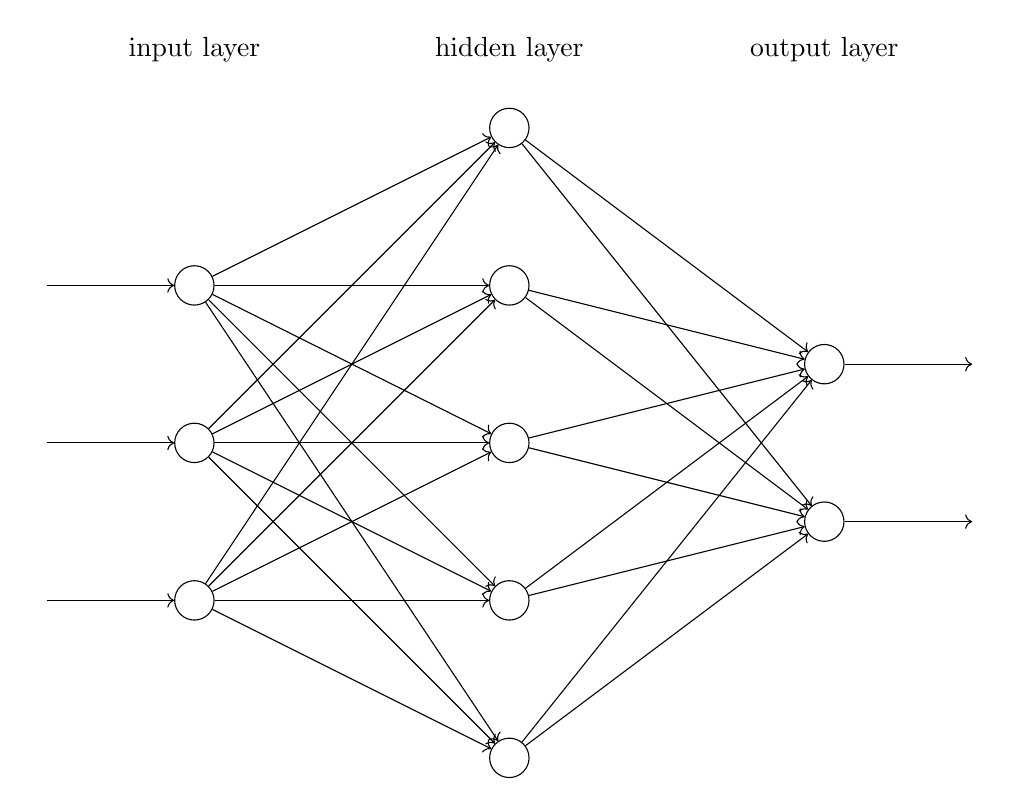
\begin{tikzpicture}[dot/.style={circle,draw,minimum size = .5cm}]
		\node at(-4,5) {input layer};
		\node at(0,5) {hidden layer};
		\node at(4,5) {output layer};

		\node at(6,1) (oo1) {};
		\node at(6,-1) (oo2) {};

		\node at (4,1) [dot] (o1) {}
			edge[->] (oo1);
		\node at (4,-1) [dot] (o2) {}
			edge[->] (oo2);

		\node at (0,4) [dot] (h1) {}
			edge[->] (o1)
			edge[->] (o2);
		\node at (0,2) [dot] (h2) {}
			edge[->] (o1)
			edge[->] (o2);
		\node at (0,0) [dot] (h3) {}
			edge[->] (o1)
			edge[->] (o2);
		\node at (0,-2) [dot] (h4) {}
			edge[->] (o1)
			edge[->] (o2);
		\node at (0,-4) [dot] (h5) {}
			edge[->] (o1)
			edge[->] (o2);

		\node at (-4,2) [dot] (i1) {}
			edge[->] (h1)
			edge[->] (h2)
			edge[->] (h3)
			edge[->] (h4)
			edge[->] (h5);
		\node at (-4,0) [dot] (i2) {}
			edge[->] (h1)
			edge[->] (h2)
			edge[->] (h3)
			edge[->] (h4)
			edge[->] (h5);
		\node at (-4,-2) [dot] (i3) {}
			edge[->] (h1)
			edge[->] (h2)
			edge[->] (h3)
			edge[->] (h4)
			edge[->] (h5);

		\node at(-6,2) (ii1) {}
			edge[->] (i1);
		\node at(-6,0) (ii2) {}
			edge[->] (i2);
		\node at(-6,-2) (ii3) {}
			edge[->] (i3);
	\end{tikzpicture}
\end{center}
\caption {Schema of a MLP or feedforward neural network.}
\label{fig:mlp}
\end{figure} % }}}

A MLP can also be represented as a statistical model
$f(\mathbf{x};\mathbf{\theta})$.
Computing $f(\mathbf{x})$---also called \textit{inference} or the
\textit{forward pass}---can be described as a layer-wise composition
of functions $f^{(1)}, f^{(2)}, \dots, f^{(l)}$, each function
$f^{(i)}, i < l$ being a hidden layer and $f^{(l)}$ being the output
layer.
The perceptron has the weight vector $\mathbf{w}$ and the bias
$b$ as its parameters (see Equation~\ref{eq:perceptron}).
The parameters of a layer are the combination of
$\mathbf{w}$ and $b$ for each of its perceptrons.
For example, if the first hidden layer contains $m$ perceptrons and
$\mathbf{x}$ is a $n$-vector, then the parameters of $f^{(1)}$ would
be a matrix $\mathbf{W}: n \times m$ and a $m$-vector $\mathbf{b}$.
The output of layer $f^{(1)}$ would be a $m$-vector computed as
follows:
\begin{align}
  f^{(1)}(\mathbf{x}; \mathbf{W}, \mathbf{b}) =
  g(\mathbf{W}^\top\mathbf{x} + \mathbf{b}).
\end{align}
The second layer takes the output of the first and so forth.
The forward pass of the MLP is computed as:
\begin{align}
  y = f^{(l)}(f^{(l-1)}(\dots f^{(1)}(\mathbf{x}))).
\end{align}

The backpropagation algorithm is a way to train the parameters of a
MLP (or other deep learning models) so that it approximates the
unknown function $f^*$ which generates the labels of the examples
we have in our data set.
The data set used for training a model is called the \textit{training
set}.
In addition to the training set there normally exists a
\textit{test set} with examples the model has not seen before
(examples not in the training set).
The test set is used to determine the generalization performance of
the model.
Backpropagation is an algorithm that allows to train a deep learning
model with \textit{(stochastic or batch) gradient descent}.
For example, $\hat{y} = f(\mathbf{x})$ and $y$ is the true label
($y$ and $\hat{y}$ are $k$-vectors), the error of $f$ is computed
using a \textit{loss function} $L$, for example mean squared error:
$1/k \sum_{i=1}^{k}(y_k - \hat{y}_k)^2$.
In order to get the \textit{gradients} of the weights of the output
layer we calculate the derivative of the loss according to each weight
$w_{ij}$ in $\mathbf{W}$ with the chain rule:
\begin{align}
  \label{eq:chain_rule}
  \frac{\delta L}{\delta w_{ij}} =
    \frac{\delta L}{\delta g}
    \frac{\delta g}{\delta h}
    \frac{\delta h}{\delta w_{ij}},
\end{align}
$h$ being $\mathbf{W}^\top f^{(l-1)} + \mathbf{b}$.

$w_{ij}$ is updated by performing some form of gradient descent:
\begin{align}
  \label{eq:sgd}
  w_{ij}^+ = w_{ij} - \mu \sum_{k=1}^{m} \frac{\delta L_k}{\delta w_{ij}}.
\end{align}
Which kind of gradient descent depends on $m$.
$m$ represents the amount of training examples seen, before the
weights are updated.
If $m$ equals one, (\ref{eq:sgd}) would be called stochastic gradient
descent.
If $m$ would encompass the whole training set, the equation would
be gradient descent.
Is $m$ somewhere in-between one and the whole training set, one
speaks of batch or mini-batch gradient descent.
A deep learning model is normally trained by passing the whole
training set multiple times through the model.
Each pass over the whole training set is called an \textit{epoch}.
$\mu$ in (\ref{eq:sgd}) is called the \textit{learning rate}.

The same procedure is applied to the following hidden layers.
The total loss of the next hidden layer is given as:
\begin{align}
  L^{(l-1)} = \sum_{i=1}^n\frac{\delta L}{\delta f^{(l - 1)}_i} =
  \sum_{i=1}^n\frac{\delta L}{\delta g}
    \frac{\delta g}{\delta h}
    \frac{\delta h}{\delta f^{(l - 1)}_i},
\end{align}
$f^{(l-1)}_i$ being the $i$-th perceptron of the hidden layer $l-1$.

\citet{hornik_et_al_1989} demonstrated that a non-linear MLP
(the activation functions are non-linear transformations of
$h(x) = \mathbf{W}^\top\mathbf{x} + \mathbf{b}$) can overcome the
famous XOR problem of a single layer perceptron demonstrated in
\citet{minsky_et_al_1969}.
Another major contribution of the phase of connectionism was the
neocognitron \citep{fukushima_1980}, the origin of today's
\textit{convolutional neural networks} (CNNs)---which are the
state-of-the-art approach for building computer vision models---and
the application of the backpropagation algorithm to fully automate the
training of CNNs \citep{lecun_et_al_1989}.

\citet{goodfellow_et_al_2016} claims that the third and current phase
of deep learning---where the name deep learning was
established---starts with \citet{hinton_et_al_2006} describing a new
learning algorithm called greedy layer-wise pretraining, which they
applied to deep belief networks.
Greedy layer-wise pretraining was soon generalized to work with other
deep artificial neural network architectures
\citep{renzato_et_al_2006, bengio_et_al_2007}.
While these papers may have resulted in the term deep learning,
they were not the reason for the resurrected interest in this
methodology.
The two most important factors are the increase of available data
and computation.
The former enables better generalization
\citep{goodfellow_et_al_2016}, while the latter allows
training bigger models (more hidden layers---the \textit{depth} of the
neural networks increased) which can solve more complex problems
\citep{bengio_et_al_2007a, goodfellow_et_al_2016}.

Like the perceptron, ``neurons'' in a \textit{convolutional layer}
are inspired by findings of neuroscientists.
In this case by research done by Hubel and Wiesel about the
mammalian visual cortex
\citep{hubel_et_al_1959, hubel_et_al_1962, hubel_et_al_1968}.
CNNs are just deep learning models which have at least one
convolutional layer. They are applied to problems which have a
grid-like topology, like time-series (1D), images (2D) or videos (3D)
\citep{goodfellow_et_al_2016}.

Unlike dense layers of perceptrons, convolutional layers do not apply
a full matrix multiplication $\mathbf{W}^\top\mathbf{x}$ but instead
a linear operation $*$ called convolution.
A one dimensional discrete convolution can be described as:
\begin{align}
  \label{eq:conv}
  s(i) = (x * w)(i) = \sum_n x(i + n)w(n).
\end{align}
Equation~\ref{eq:conv} is not really a convolution but is referred to
as \textit{cross-correlation}.
Unlike true convolution, cross-correlation is not commutative
\citep{goodfellow_et_al_2016}.
However, commutativity is not a factor in practice, so many deep
learning libraries, like Keras \citep{keras} or the prototype
developed for this thesis implement cross-correlation rather than true
convolution.
Convolution will refer to cross-correlation below.

In the case of deep learning, $x$ is a $n$D array called the
\textit{input} and $w$ is another $n$D array referred to as the
\textit{kernel}. The kernel elements are the trainable parameters
\citep{goodfellow_et_al_2016}.
In Equation~\ref{eq:conv}, $x$ and $w$ are one dimensional.
If we let $x$ be a $m$-vector, the function $x(i)$ is defined as:
\begin{align}
  \label{eq:valid_conv}
  x(i) = \begin{cases}
    x_i &\text{if } 1 \leq i \leq m \\
    0 &\text{otherwise.}
  \end{cases}
\end{align}
$n$ is the size of the kernel in the first dimension.
Figure~\ref{fig:conv_op} shows an example of how the output of a
1D convolutional layer is computed.
Figure~\ref{fig:cnn} shows the schema of the convolutional
layer performing the operation from Figure~\ref{fig:conv_op}.
The result of a convolution can be transformed by an activation
function like the perceptron and the concept of the bias applies also.

\begin{figure} % {{{
\begin{center}
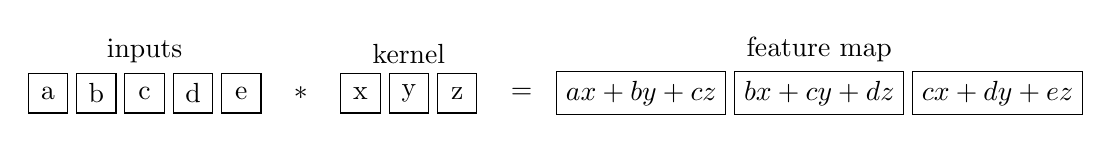
\begin{tikzpicture}[box/.style={rectangle,draw, minimum size=.5cm}]
  \node[box] at (0,0) (a) {a};
  \node[right=.1 of a, box] (b) {b};
  \node[right=.1 of b, box, label=inputs] (c) {c};
  \node[right=.1 of c, box] (d) {d};
  \node[right=.1 of d, box] (e) {e};

  \node[right=.9 of d] {$*$};

  \node[right=1 of e, box] (x) {x};
  \node[right=.1 of x, box, label=kernel] (y) {y};
  \node[right=.1 of y, box] (z) {z};

  \node[right=.3 of z] {$=$};

  \node[right=1 of z, box] (fst) {$ax + by + cz$};
  \node[right=.1 of fst, box, label=feature map] (snd)
    {$bx + cy + dz$};
  \node[right=.1 of snd, box] (trd) {$cx + dy + ez$};
\end{tikzpicture}
\end{center}
\caption{Example of a 1D cross-correlation operation with a kernel
  size of three, a single channel, a single filter, a stride of one
  and valid padding.}
\label{fig:conv_op}
\end{figure} % }}}

\begin{figure} % {{{
\begin{center}
	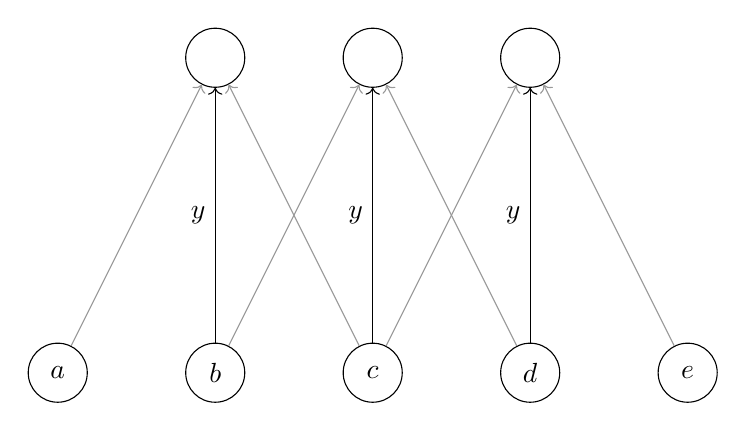
\begin{tikzpicture}[rotate=90, dot/.style={circle,draw,minimum size = .75cm}]
		\node at (0,2) [dot] (h2) {};
		\node at (0,0) [dot] (h3) {};
		\node at (0,-2) [dot] (h4) {};

		\node at (-4,4) [dot] (i1) {$a$}
			edge[black!40, ->] (h2);
		\node at (-4,2) [dot] (i2) {$b$}
			edge[->] (h2)
			edge[black!40, ->] (h3);
		\node at (-4,0) [dot] (i3) {$c$}
			edge[black!40, ->] (h2)
			edge[->] (h3)
			edge[black!40, ->] (h4);
		\node at (-4,-2) [dot] (i4) {$d$}
			edge[black!40, ->] (h3)
			edge[->] (h4);
		\node at (-4,-4) [dot] (i5) {$e$}
			edge[black!40, ->] (h4);

    \node[left] at (-2,2) {$y$};
    \node[left] at (-2,0) {$y$};
    \node[left] at (-2,-2) {$y$};
	\end{tikzpicture}
\end{center}
\caption {Schema for the convolutional layer performing the
  convolution shown in Figure~\ref{fig:conv_op}. Each neuron
  represents one convolution. The schema shows the
  property of shared weights and sparse
  connectivity \citep{goodfellow_et_al_2016}. The black edges
  all have the same associated weight $y$, while one can see that
  there are much less edges compared to a dense layer shown in
  Figure~\ref{fig:mlp}.}
\label{fig:cnn}
\end{figure} % }}}

Normally a convolutional layer does not consist of a single
convolution, but applies multiple kernels to the output of the
previous layer.
A single convolution is called a \textit{filter} and a layer
consists of a predefined number of filters, each with its own kernel
(and optionally a bias) \citep{brownlee_2019}.
The output of a convolutional layer is often called a
\textit{feature map} \citep{goodfellow_et_al_2016}.
Even though an image may seem to be a two dimensional structure of
pixels, in most cases it is actually three dimensional, the third
dimension being the RGB color values for each pixel.
The third dimension of the three RGB colors are called the
\textit{channels} \citep{goodfellow_et_al_2016}.
For example, we have a data set of images with $256\times256$
pixels and three channels (red, green and blue).
We pass the image to a convolutional layer with a $3\times3$ kernel
shape and $64$ filters.
A kernel consists of 18 elements, the kernel size (for the two
spatial dimensions) times the three channels of each pixel.
The shape of the feature map of that layer---if we assume ``same''
padding (see below)---would be $256\times256\times64$, so the
next layer would have 64 channels.

There are two more notable concepts of convolutional layers:
\textit{stride} and \textit{padding}.
The former refers to skipping convolutions in order to reduce the
computational cost at the expense of less exact feature extraction
(patterns may not be detected by the model due to the increased
inaccuracy).
The latter is a way of dealing with vanishing spatial dimensions of
the feature map if we only perform convolutions on ``valid'' inputs
($1 \leq i \leq m$ in Equation~\ref{eq:valid_conv}).
``Valid'' padding refers to the fact that the input has no padding.
The feature map of the convolutional layer will have
its kernel size minus one less neurons than its input
(see Figure~\ref{fig:cnn}).
``Same'' padding would be to add enough zeros evenly above and below
the valid input (along each spatial dimension) so that the feature map
of the convolutional layer will have the same spatial dimensions as
its input (see Figure~\ref{fig:padding} \citep{goodfellow_et_al_2016}.

\begin{figure} % {{{
\begin{center}
	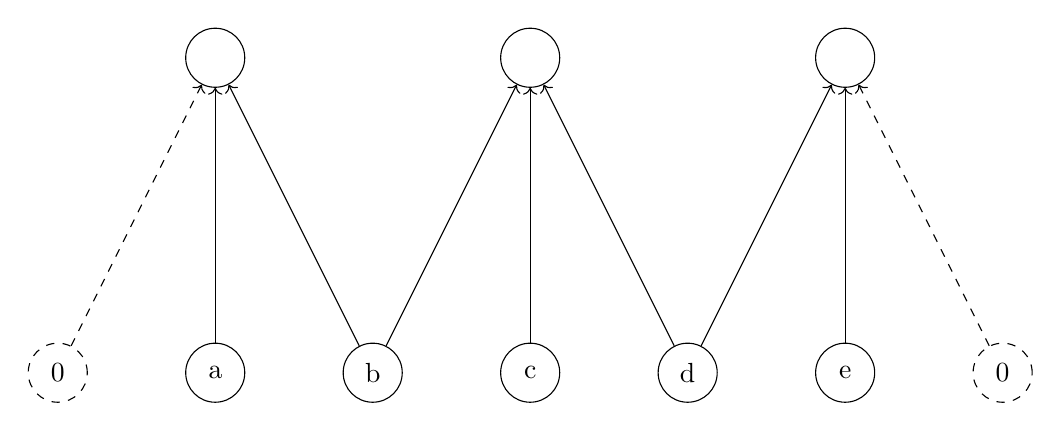
\begin{tikzpicture}[rotate=90, dot/.style={circle,draw,minimum size = .75cm}]
		\node at (0,4) [dot] (h1) {};
		\node at (0,0) [dot] (h3) {};
		\node at (0,-4) [dot] (h5) {};

		\node at (-4,6) [dot, dashed] (i0) {0}
			edge[->, dashed] (h1);
		\node at (-4,4) [dot] (i1) {a}
      edge[->] (h1);
		\node at (-4,2) [dot] (i2) {b}
			edge[->] (h1)
			edge[->] (h3);
		\node at (-4,0) [dot] (i3) {c}
			edge[->] (h3);
		\node at (-4,-2) [dot] (i4) {d}
			edge[->] (h3)
			edge[->] (h5);
		\node at (-4,-4) [dot] (i5) {e}
			edge[->] (h5);
		\node at (-4,-6) [dot, dashed] (i6) {0}
			edge[->, dashed] (h5);
	\end{tikzpicture}
\end{center}
\caption {Example showing a layer with same padding and a
  stride of two.}
\label{fig:padding}
\end{figure} % }}}

Along convolutional layers, CNNs often have \textit{pooling layers}.
A pooling layer summarizes locally with the goal of making the
CNN invariant to small translations of the input
\citep{goodfellow_et_al_2016}, making the model less prone to
\textit{overfitting}---the state a model is in if it performs well
on the training set but does not generalize well to unseen examples.
\textit{Max pooling}, for example, takes some local neighborhood of
the input, exactly like a convolutional layer, and returns the
maximum value of that neighborhood.

% }}}


\subsection{Benchmarking Deep Learning Systems for Computer Vision} % {{{
\label{subsec:intro_bench}

In 2010 the annual (until 2017) ImageNet Large Scale Visual
Recognition Challenge (ILSVRC) was launched and has become the most
famous benchmark for computer vision models, producing many well-known
deep learning models like AlexNet in 2012
\citep{krizhevsky_et_al_2012}, VGG16 in 2014
\citep{simonyan_et_al_2014} and the ResNet models in 2015
\citep{he_et_al_2015}.
The ILSVRC---like the name suggests---is based on the ImageNet data
set consisting of more than 14 million images
\citep{russakovsky_et_al_2015}.
One task of the ILSVRC benchmark is image classification.
During image classification the model is trained on 1000 categories
(1.2 million images), without overlapping labels (each image has a
single label, e.g.~``dog'') \citep{russakovsky_et_al_2015}.
The top-1 ($y = \text{argmax } f(\mathbf{x})$) accuracy is measured on
a test set of 150,000 images and winner is the model with the highest
top-1 accuracy.

While a benchmark like the ILSVRC produces new insights into computer
vision and keeps the community up to date on what is possible,
deep learning has another issue on which a benchmark can shed light:
training/inference speed of hardware and software systems.
The MLPerf benchmark was developed to tackle this problem, so
stakeholders can make informed decisions and to provide the
industry---like hardware vendors, cloud providers and machine learning
engineers---with a fair standard to rely on
\citep{mattson_et_al_2019}.
One task of the MLPerf training benchmark is training the ResNet-50
model (see below) on the image classification task from the ILSVRC
2012, until it reaches a top-1 accuracy of 74.9 percent.
The wallclock time is measured and serves as the result for the
benchmarked system \citep{mattson_et_al_2019}.
Currently the fastest solution, from the latest MLPerf training
benchmark v0.6, is Google's cloud system based on Tensorflow and
one TPUv3 pod (1024 TPUv3s) \citep{mlperf_2019, stone_2019}.
The benchmark we wanted to conduct in order to compare our
implementation against others, is based
on the image classification task of the MLPerf training benchmark,
making it easy to compare SpiNNaker and our prototype to other
state-of-the-art deep learning systems.

The winner of the image classification task of the ILSVRC 2015 was an
ensemble of residual nets (ResNets) introduced in
\citet{he_et_al_2015}.
The ensemble generated a top-5 accuracy (true label in the five
highest outputs of the ensemble) of 96.4 percent.
ResNets are a revolution in the sense that they are not only better
classifiers than previous models, they also can be significantly
deeper \citep{he_et_al_2015}.
\citet{he_et_al_2015} presents a 152-layer deep network, eight times
deeper than a ``very deep convolutional network'' (VGG11--VGG19)
\citep{simonyan_et_al_2014, he_et_al_2015}.
ResNets can be so deep, without losing their ability of convergence
and without degradation (saturated accuracy and higher training error
with increased depth) \citep{he_et_al_2015}, by introducing residual
blocks with shortcut connections (see Figure~\ref{fig:shortcut_conn}).
\citet{he_et_al_2015} hypothesizes that residual blocks ease the
learning of the model.
These shortcut connections do not increase the complexity of the
model. No additional parameters are added to the model and nothing
changes during backpropagation.
Only the negligible operation where $\mathbf{x}$ is added to the
output of the residual block must be performed during the forward
pass.
\citet{he_et_al_2015} shows comprehensive tests on how residual blocks
decrease degradation by comparing ResNets against their
counterparts with the same architecture, but without shortcut
connections.
The models without shortcut connections show a higher training error
than their ResNet counterpart.

\begin{figure}
  \begin{center}
    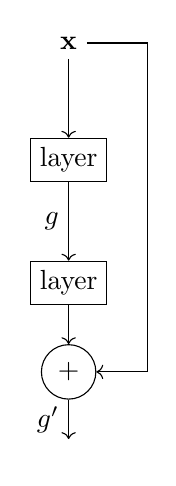
\begin{tikzpicture}
      \node[rectangle, draw] at (0, 0) (layer0) {layer};
      \node[rectangle, draw, below=1 of layer0] (layer1) {layer};
      \node[circle, draw, below=.5 of layer1] (layer_add) {$+$};
      \node[below=.5 of layer_add] (layer_out) {};
      \node[above=1 of layer0] (layer_in) {$\mathbf{x}$};

      \draw[->] (layer_in) -- (layer0);
      \draw[->] (layer0) -- node[left]{$g$} (layer1);
      \draw[->] (layer1) -- (layer_add);
      \draw[->] (layer_add) -- node[left]{$g^\prime$} (layer_out);

      \draw[->] (layer_in) -| ($(layer_add) + (1,0)$) |- (layer_add);
    \end{tikzpicture}
  \end{center}
  \caption{Schema of a residual block with two layers. $\mathbf{x}$ is
    added to the output of the last layer of the residual block,
    before the result is passed through its activation function
    $g^\prime$.}
  \label{fig:shortcut_conn}
\end{figure}

As stated above, the image classification task of the MLPerf
training benchmark is to train ResNet-50 (50, because it has 50
layers) until it reaches a top-1 accuracy of 74.9 percent on the test
set and to measure the wallclock time it took to reach that goal.
Figure~\ref{fig:resnet50_block} shows an example block from the
ResNet-50 model, while Figure~\ref{fig:resnet50} shows its
architecture.
The model takes a $224\times224\times3$ image as its input and first
passes it through a convolutional layer with a relatively big kernel
of $7\times7$ and a max pooling layer.
Both times the spatial dimensions are halved by applying a stride of
two, so the first residual block receives a $56 \times 56 \times 64$
feature map as its input.
The model consists of multiple residual blocks.
Some of them have a stride of two.
Each time the input is halved that way, channels are doubled.
This should keep computational cost the same for each block
\citep{he_et_al_2015}.

\begin{figure}
  \begin{center}
    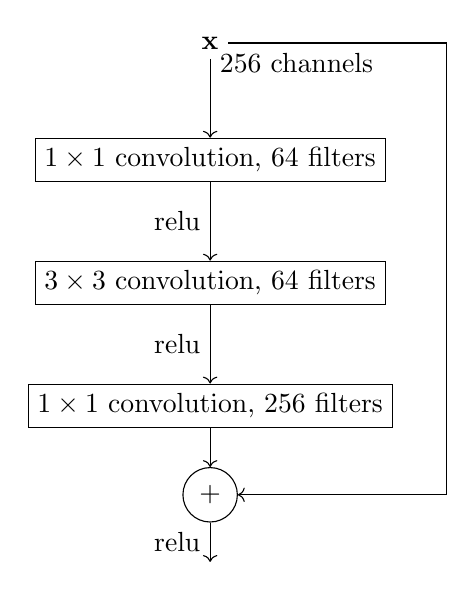
\begin{tikzpicture}
      \node[rectangle, draw] at (0, 0) (layer0)
        {$1\times1$ convolution, 64 filters};
      \node[rectangle, draw, below=1 of layer0] (layer1)
        {$3\times3$ convolution, 64 filters};
      \node[rectangle, draw, below=1 of layer1] (layer2)
        {$1\times1$ convolution, 256 filters};
      \node[circle, draw, below=.5 of layer2] (layer_add) {$+$};
      \node[below=.5 of layer_add] (layer_out) {};
      \node[above=1 of layer0] (layer_in)
        {$\mathbf{x}$};

      \draw[->] (layer_in) -- (layer0);
      \draw[->] (layer0) -- node[left]{relu} (layer1);
      \draw[->] (layer1) -- node[left]{relu} (layer2);
      \draw[->] (layer2) -- (layer_add);
      \draw[->] (layer_add) -- node[left]{relu} (layer_out);

      \draw[->] (layer_in) node[below right] {256 channels} -| ($(layer_add) + (3,0)$) |- (layer_add);
    \end{tikzpicture}
  \end{center}
  \caption{Example of a residual block in ResNet-50.}
  \label{fig:resnet50_block}
\end{figure}

\begin{figure}
  \begin{center}
    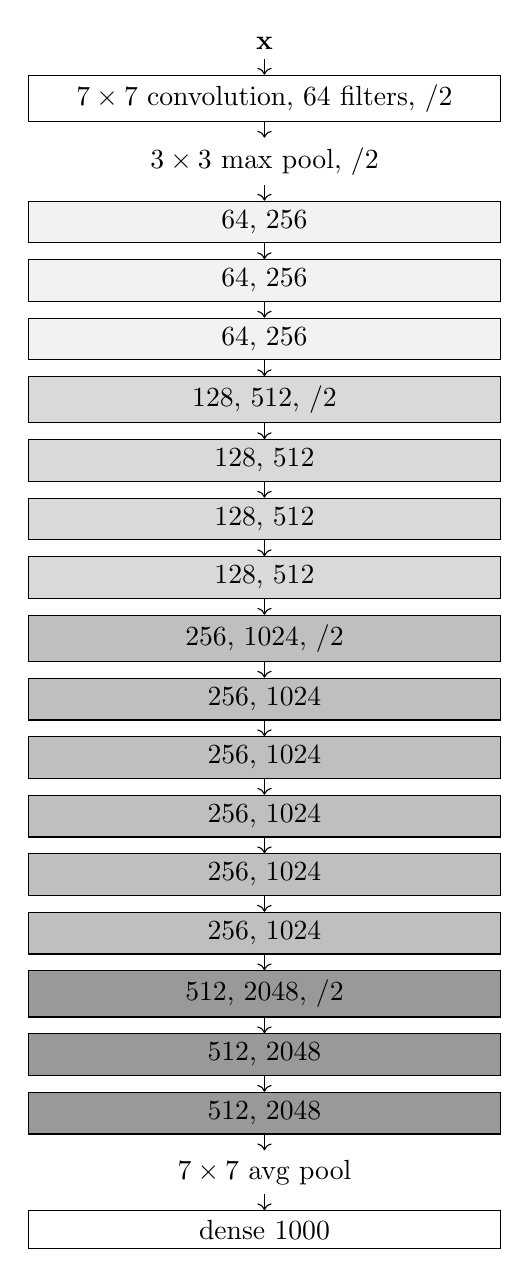
\begin{tikzpicture}[block/.style={rectangle, draw, minimum width=6cm}]
      \node[block, fill=black!5] at (0, 0) (block0) {64, 256};
      \node[block, fill=black!5, below=.2 of block0] (block1) {64, 256};
      \node[block, fill=black!5, below=.2 of block1] (block2) {64, 256};

      \node[block, fill=black!15, below=.2 of block2] (block3) {128, 512, /2};
      \node[block, fill=black!15, below=.2 of block3] (block4) {128, 512};
      \node[block, fill=black!15, below=.2 of block4] (block5) {128, 512};
      \node[block, fill=black!15, below=.2 of block5] (block6) {128, 512};

      \node[block, fill=black!25, below=.2 of block6] (block7) {256, 1024, /2};
      \node[block, fill=black!25, below=.2 of block7] (block8) {256, 1024};
      \node[block, fill=black!25, below=.2 of block8] (block9) {256, 1024};
      \node[block, fill=black!25, below=.2 of block9] (block10) {256, 1024};
      \node[block, fill=black!25, below=.2 of block10] (block11) {256, 1024};
      \node[block, fill=black!25, below=.2 of block11] (block12) {256, 1024};

      \node[block, fill=black!40, below=.2 of block12] (block13) {512, 2048, /2};
      \node[block, fill=black!40, below=.2 of block13] (block14) {512, 2048};
      \node[block, fill=black!40, below=.2 of block14] (block15) {512, 2048};

      \node[below=.2 of block15] (pool2) {$7\times7$ avg pool};
      \node[block, below=.2 of pool2] (dense) {dense 1000};

      \node[above=.2 of block0] (pool1) {$3 \times 3$ max pool, /2};
      \node[block, above=.2 of pool1] (conv1)
        {$7\times7$ convolution, 64 filters, /2};
      \node[above=.2 of conv1] (x) {$\mathbf{x}$};

      \draw[->] (block0) -- (block1);
      \draw[->] (block1) -- (block2);
      \draw[->] (block2) -- (block3);
      \draw[->] (block3) -- (block4);
      \draw[->] (block4) -- (block5);
      \draw[->] (block5) -- (block6);
      \draw[->] (block6) -- (block7);
      \draw[->] (block7) -- (block8);
      \draw[->] (block8) -- (block9);
      \draw[->] (block9) -- (block10);
      \draw[->] (block10) -- (block11);
      \draw[->] (block11) -- (block12);
      \draw[->] (block12) -- (block13);
      \draw[->] (block13) -- (block14);
      \draw[->] (block14) -- (block15);

      \draw[->] (x) -- (conv1);
      \draw[->] (conv1) -- (pool1);
      \draw[->] (pool1) -- (block0);
      \draw[->] (block15) -- (pool2);
      \draw[->] (pool2) -- (dense);
    \end{tikzpicture}
  \end{center}
  \caption{Schema of ResNet-50. Each block in the middle represents
    one residual block shown in Figure~\ref{fig:resnet50_block}.
    The first number shows the amount of filters the first two layers
    of a block have, while the second number shows the filters of the
    last layer of the block. $/2$ indicates that a stride of two is
    applied (spatial dimensions are halved---each convolutional and
    pooling layer has ``same'' padding). Whenever the filters are
    doubled (indicated by the varying grey scales), the shortcut layer
    is linearly projected to match the higher channels.}
  \label{fig:resnet50}
\end{figure}

% }}}


\subsection{SpiNNaker as a Neuromorphic Computer Architecture} % {{{
\label{subsec:intro_spinn}

Spiking Neural Network Architecture (SpiNNaker, for short) is a
massively parallel neuromorphic computer system designed to run
spiking neural networks with up to one billion neurons (and a trillion
synapses) in real-time \citep{painkras_et_al_2013}.
As stated in Section~\ref{sec:intro}, neuromorphic computing is
the approach of developing hardware inspired by the biological
nervous system \citep{mead_1989}.
Today, neuromorphic computer architectures range from very fast and
energy efficient but inflexible direct electronic models
(neurons in hardware) \citep{indiveri_et_al_2011} to very flexible but
energy demanding systems based on common consumer hardware and
software (neurons in software) \citep{plesser_et_al_2007}.
SpiNNaker sits somewhere in between.
On the one hand, flexibility is achieved by implementing neurons in
software.
On the other hand, speed is achieved by massive-parallelism and
energy efficiency by using energy efficient processors, rather than
fast ones \citep{furber_et_al_2020}.

The SpiNNaker system's basic building block is the SpiNNaker chip,
a multiprocessor chip consisting of 18 ARM968 cores
\citep{furber_et_al_2020} and a
Network-on-Chip (NoC) system for communication between the cores
\citep{furber_et_al_2007}.
Each core can run up to 1000 spiking neurons, which communicate with
each other over spikes---small packages with a maximum size of 72 bits
which are sent over the NoC \citep{furber_et_al_2007, spinnaker_2020}.
Each core has a 64 Kb DTCM---data tightly-coupled memory---for the
application data and fast access to it.
The 32 Kb ITCM stores the instructions executed by the core
\citep{furber_et_al_2020}.
All cores on a chip share access to 128 Mb SDRAM---synchronous
dynamic random access memory---which has a higher capacity than
DTCM but is also a lot slower
\citep{furber_et_al_2020, spinnaker_2020a}.

By today's standards 18 cores do not qualify as a massively-parallel
system.
Therefore, a SpiNNaker machine consists of multiple chips connected
together in a 2D triangular (six edges per router instead of four)
torus \citep{furber_et_al_2020}.
The biggest SpiNNaker machine is the SpiNNaker1M supercomputer in
Manchester with over one million cores.
The SpiNNaker1M consists of 10 cabinets, each with five card frames
holding 24 SpiNN-5 boards.
A SpiNN-5 board has 48 SpiNNaker chips, which means the SpiNNaker1M
has 1,036,800 theoretical cores, assuming no faulty cores
\citep{furber_et_al_2020}.\footnote{During the introduction of the
  SpiNNaker1M 1,010,285 cores were working \citep{uoecompsci_2019}.}
Images of the SpiNNaker hardware can be found in
Appendix~\ref{sec:spinn_photos}.

SpiNNaker is quite different from common deep learning accelerators,
like general purpose graphics processing units (GPGPUs) or Google's
TPU \citep{jouppi_et_al_2017}.
Common deep learning libraries like Tensorflow
\citep{abadi_et_al_2015}, Keras \citep{keras} or PyTorch
\citep{paszke_et_al_2019} implement
deep learning on a layer basis, which means by multiplying
\textit{tensors} ($n$D arrays), rather than implementing deep learning
on a neuron level \citep{goodfellow_et_al_2016}.
Therefore, the common industry approach to building hardware
accelerators for deep learning is to facilitate fast matrix
multiplication, which represents the majority of computation needed
for training and inference.
The leading systems, when it comes to throughput and speed according
to the MLPerf training benchmark \citep{mlperf_2019}, are Google's
TPU \citep{jouppi_et_al_2017} and NVIDIA's GPU architecture
Volta \citep{durant_et_al_2017}.
Volta's successor Ampere was released in 2020, which, according to
NVIDIA, is much more powerful \citep{krashinsky_et_al_2020}.
Both architectures leverage instruction level parallelism, sacrificing
significant chip space for specialized units performing a
fused multiply-add-accumulate matrix operation (MAC).
NVIDIA calls these units tensor cores. The Tesla V100 has 640 tensor
cores, each performing one $4\times 4$ MAC per clock cycle, a
theoretical peak performance of 125 terraflop/s
\citep{markidis_et_al_2018}.
The TPUv1 comes with $256\times256$ MACs performing 8 bit (unsigned)
integer operations \citep{jouppi_et_al_2017}.
The TPUv2 added support for mixed precision floating point operations
(16 bit multiply with 32 bit add and accumulate, same as the
tensor core of the Volta architecture)
\citep{kennedy_2017, markidis_et_al_2018}.
The SpiNNaker cores do not have a MAC unit, being designed to run
spiking neurons efficiently, rather than lots of matrix
multiplications.
That means the prototype presented in Section~\ref{sec:SpiDNN} must
put more focus on leveraging SpiNNaker's massive parallelism, rather
than relying on fast instruction level parallelism.
For example with optimized domain decomposition and smarter algorithms
than matrix multiplication.

% }}}

% }}}


\section{Related Work} % {{{
\label{sec:related_work}

Like \citet{gomes_2017} states, implementing deep learning on
neuromorphic chips has been a goal for some time.
This section will outline two approaches to implementing deep learning
models on neuromorphic hardware.
One being the SNN toolbox \citep{rueckauer_et_al_2017}, the other
being an implementation of CNNs on IBM's TrueNorth system
\citep{esser_et_al_2016}.

The SNN toolbox takes pre-trained deep learning models and translates
them into spiking neural networks.
Its front-end supports a wide range of different input formats from
various deep learning libraries, including Keras, Tensorflow, PyTorch
and Caffe \citep{jia_et_al_2014}, while its back-end supports
different spiking neural network simulators like Brian2
\citep{stimberg_et_al_2019}.
The back-end also supports the simulator-independent language PyNN
\citep{davison_et_al_2009}, enabling running the converted models
on SpiNNaker, which supports PyNN as its front-end for spiking neural
networks.
Furthermore, direct mappings to other neuromorphic
computers like Intel's Loihi \citep{davies_et_al_2018} are supported
by the back-end \citep{snn_toolbox_2020}.
The SNN toolbox supports complex CNNs like VGG16 or Inception-v3
\citep{szegedy_et_al_2015, rueckauer_et_al_2017}.
\citet{rueckauer_et_al_2017} shows that using the converted version of
LeNet \citep{lecun_et_al_1989} on the MNIST data set
\citep{lecun_et_al_2020} and BinaryNet \citep{courbariaux_et_al_2016}
on CIFAR-10 \citep{krizhevsky_2009} requires half the
operations of the original CNNs without considerable loss in
accuracy.
Unfortunately, for bigger problems, namely VGG16 and Inception-v3 on
the ImageNet data set, the converted models have a much lower accuracy
than their original counterpart (63.9 percent accuracy for the
original VGG16 and only 49.6 for the converted model)
\citep{rueckauer_et_al_2017}.
Another caveat of the SNN toolbox is the fact that it only supports
inference and not training.
Training is the far more complex task computationally.

IBM's TrueNorth neuromorphic architecture has the goal of
achieving energy efficiency and performance through scalability,
similar to SpiNNaker.
\citet{esser_et_al_2016} presents Eedn (energy-efficient deep
neuromorphic networks).
Eedn is an approach to generating CNNs on the TrueNorth system,
enabling both inference and training.
TrueNorth---unlike SpiNNaker---uses one bit spikes
\citep{esser_et_al_2016}, which means it is substantially different
from contemporary consumer hardware and deep learning accelerators.
Eedn is needed to translate the CNN in order to make it run on
TrueNorth.
SpiNNaker on the other hand, as stated above, is only a collection
of low power ARM cores connected over a NoC.
Spikes on SpiNNaker are communicated with small multicast packets
(up to 72 bits, see Section~\ref{subsec:intro_spinn})
\citep{furber_et_al_2020}.
These packets can be used to transfer any information from one core
to another.
This makes it much easier to implement deep learning on SpiNNaker,
because focus lies more on how to deconstruct the model and map it
onto the cores, rather than having to translate the model into a
SpiNNaker-specific format.
Nonetheless, Eedn models show promising results.
\citet{esser_et_al_2016} presents tests on 6 well known,
industry-strength data sets with the Eedn models having approximately
the same accuracy as the original models.
The throughput of the TrueNorth system is promising as well.
\citet{esser_et_al_2016} shows that TrueNorth is able to process
between 1,200 and 2,600 $32\times32\times3$ images per second.

% }}}


\section{Deep Learning on SpiNNaker} % {{{
\label{sec:SpiDNN}

This section will describe the developed deep learning prototype in
detail.
While Section~\ref{subsec:intro_spinn} gave a short overview over the
SpiNNaker hardware, Section~\ref{subsec:spinn_toolchain} will present
a short introduction to the SpiNNaker software toolchain and
programming model.
Section~\ref{subsec:SpiDNN_arch} will present the architecture of the
prototype.
Lastly, Section~\ref{subsec:problems} will describe the
hardships and problems encountered and mistakes made during the
development process.


\subsection{The SpiNNaker Programming Model} % {{{
\label{subsec:spinn_toolchain}

Parallel programming is hard \citep{lee_2011}, especially on novel
hardware architectures like SpiNNaker \citep{brown_et_al_2015}.
SpiNNaker provides layers of software abstractions over the hardware
to make programming and exploiting the capabilities of it as easy as
possible \citep{furber_et_al_2020}.

The SpiNNaker hardware is designed to tackle problems which can be
decomposed into many small, autonomous units without a central
computational overseer \citep{brown_et_al_2015}.
These problems are commonly known as embarrassingly parallel problems
\citep{foster_1995}.
The software toolchain lets the user describe their program as a
graph.
Each vertex of the graph represents one unit of computation
(e.g.\ a bunch of spiking neurons or a perceptron in our case)
and directed edges represent the communication between the units
\citep{furber_et_al_2020}.

There are two type of graphs, application graphs and machine graphs.
A vertex in the machine graph, referred to as a machine vertex, is
directly mapped to a single SpiNNaker core.
An application graph is an abstraction over a machine graph.
Application vertices have a number of atoms, each being an atomic unit
of computation.
The atoms of an application vertex are distributed onto machine
vertices, such that each machine vertex contains a disjunct subset
of the atoms of the corresponding application vertex.
This makes programming and scaling easier and also facilitates proper
resource exploitation.
For example by mapping 1,000 small spiking
neurons---atoms of a neuron population represented as a application
vertex---onto a single core, instead of having them distributed across
1,000 cores, which would be the case if they were to be implemented
directly as machine vertices \citep{furber_et_al_2020}.
For the prototype we used a machine graph, since it is easier to
implement.
Less code is required and the difficulties of multiplexing and
demultiplexing are avoided.
The development process was guided by the UNIX rule of optimization:
prototype before polishing \citep{raymond_2003}, or in Donald Knuth's
words: ``premature optimization is the root of all evil''
\citep{knuth_1974}.

The SpiNNaker toolchain is mostly written in the Python programming
language.
The SpiNNaker machine is connected to a host device via Ethernet
\citep{rowley_et_al_2019}.
In order to execute a program on SpiNNaker, one writes a Python
script which generates a graph.
It must be either an application graph or a machine graph.
Machine vertices cannot be added to an application graph and vice
versa.
The toolchain---running on the host which also executes the script
generating the graph---takes a lot of boilerplate away from the user
and takes care of the execution of the program on the connected
SpiNNaker machine.
The toolchain goes through a stage of mapping the graph onto the
available cores, before data generation (where e.g.\ parameters of the
vertex are loaded into SDRAM, so that the vertex on the machine is
able to access them) and finally loading and running the
application \citep{furber_et_al_2020}.

Each vertex is represented as a Python object---instantiated from the
appropriate classes---and has an associated binary---the program to
be executed by the machine \citep{furber_et_al_2020}.
The source code of the binary to be executed on the machine is written
in the C programming language and compiled with the gcc compiler from
the GNU ARM embedded toolchain \citep{arm_2020, rowley_et_al_2019}.
Machine vertices are not common C programs.
They do not own the control flow but instead are event-based, like
the ECMAScript programming language \citep{ecma_2020}.
The SpiNNaker1 API provides the operating system executing the vertex
and serves as the mechanism for registering software callback
functions, triggered when a certain event occurs
\citep{furber_et_al_2020}.
The two events used by the vertices of this prototype were:
(\romannumeral 1) receiving a packet and (\romannumeral 2) a
periodic update event, called every $x$ microseconds.
During testing, we set the update event to be called every five
milliseconds, which is rather slow but true to our design philosophy
of prototyping before polishing.

\begin{figure} % {{{
\begin{center}
  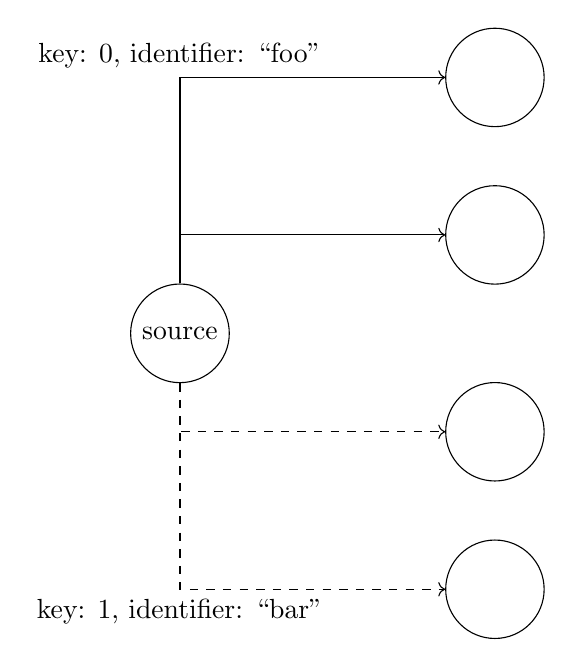
\begin{tikzpicture}[dot/.style={circle, draw, minimum size=1.25cm}]
    \node[dot] at (0, 0) (source) {source};

    \node[dot] at (4, 3.25) (dest1) {};
    \node[dot] at (4, 1.25) (dest2) {};
    \node[dot] at (4, -1.25) (dest3) {};
    \node[dot] at (4, -3.25) (dest4) {};

    \draw[->] (source) |-
      node[above]{key: 0, identifier: ``foo''} (dest1);
    \draw[->] (source) |- (dest2);

    \draw[->, dashed] (source) |- (dest3);
    \draw[->, dashed] (source) |-
      node[below]{key: 1, identifier: ``bar''} (dest4);
  \end{tikzpicture}
\end{center}
\caption{Example of a machine vertex ``source'' connected to four
  other machine vertices over two outgoing edge partitions.}
\label{fig:partitions}
\end{figure} % }}}

Machine vertices communicate with each other via MC (multicast)
packets.
A MC packet has two or three segments:
(\romannumeral 1) one control byte, (\romannumeral 2) 4 byte key
and (\romannumeral 3) optionally 4 byte payload.
This makes a MC packet either 40 or 72 bits long
\citep{furber_et_al_2020}.
A MC packet is sent via the directed edges between vertices.
Each edge has an associated outgoing edge partition.
An outgoing edge partition has one source vertex and $n$ destination
vertices and---in the case of the machine graph---one unique
routing key (allocated by the toolchain).
The routing key---a 32 bit unsigned integer---is unique in the sense
that no other outgoing edge partition will have the same key.
Otherwise routing would fail, because packets would be send
to the wrong destinations or dropped when no matching router entry for
the key is found.
If the source vertex sends a MC packet it uses the key of the
outgoing edge partition.
The packet will reach all destination vertices of the outgoing edge
partition.
A vertex can have multiple outgoing edge partitions, as is shown in
Figure~\ref{fig:partitions} \citep{furber_et_al_2020}.
If the source vertex from Figure~\ref{fig:partitions} sends a MC
packet with key zero, the two upper vertices will receive the
packet, whereas with key one the two lower vertices would receive
the packet.

The toolchain offers support for live IO, enabling external devices
(like robots, or in our case the host) to interact with the
application running on SpiNNaker.
Interaction happens, again, via MC packets\footnote{%
  MC packets are the abstraction presented to the user. In fact,
  communication between the host and the SpiNNaker machine are handled
  by the EIEIO (external internal event input output) protocol
  \citep{rast_et_al_2015}.
  The EIEIO protocol sits on-top of the SpiNNaker-internal SDP
  (SpiNNaker datagram protocol), which itself sits on-top of UDP
  \citep{furber_et_al_2014}.
}
by adding extra vertices for input and output to the graph.
Live input is enabled by the \texttt{ReverseIPTagMulticastSource}
(RIPTMCS) machine vertex and live output by the
\texttt{LivePacketGatherer} (LPG) \citep{furber_et_al_2020}.
The toolchain provides a \texttt{LiveEventCon\-nection} for the
external device, which supplies the appropriate abstractions over the
networking.
Like the SpiNNaker1 API, the \texttt{Live\-Event\-Con\-nection}
provides an event-based interface with callbacks.

% }}}


\subsection{The Prototype} % {{{
\label{subsec:SpiDNN_arch}

The underlying assumption made for developing the prototype was,
that because SpiNNaker was designed to run spiking neurons, it would
be a natural fit to implement deep learning on a neuron level as well.
Besides that, neurons are an easy-to-understand abstraction over the
mechanisms of deep learning and rather straightforward to implement.
This design decision was made against the trend of both deep learning
research and state-of-the-art deep learning libraries.
The former more commonly abstracts over layers while the latter
implements deep learning as a computational graph
\citep{goodfellow_et_al_2016}.
Problems with this assumption are discussed in
Section~\ref{subsec:problems}.
The API of the prototype was designed to resemble the API of the Keras
deep learning library \citep{keras}.
An example comparison can be seen in
Listing~\ref{lst:spiDNN_vs_keras}.

\begin{figure} % {{{
\begin{lstlisting}[language=Python, caption={Example code comparing
  inference with Keras to inference with the prototype. The code would
  result in a model akin to the one shown in
  Figure~\ref{fig:spiDNN_arch}.}, captionpos=b,
  label=lst:spiDNN_vs_keras, numbers=left]
import tensorflow as tf
import numpy as np

# prototype library
from spiDNN import Model
from spiDNN.layers import Input, Dense

# random test set
X = np.random.rand(500, 64)

# the keras model
keras_model = tf.keras.Sequential()
keras_model.add(tf.keras.layers.Dense(128, input_shape=(64,)))
keras_model.add(tf.keras.layers.Dense(128, activation=`relu'))
keras_model.add(tf.keras.layer.Dense(10, activation=`softmax'))

# the equivalent model for SpiNNaker
spinn_model = Model()
spinn_model.add(Input(64))
spinn_model.add(Dense(128))
spinn_model.add(Dense(128, activation=`relu'))
spinn_model.add(Dense(10, activation=`softmax'))

# this call ensures both models have the same parameters
model.set_weights(keras_model.get_weights())

# predict the results for the random test set (with random weights)
p_ = kmodel.predict(X)
p = model.predict(X)

error = np.absolute(p - p_)

# difference in prediction can happen, due to floating point errors
assert np.amax(error) < 1e-4
\end{lstlisting}
\end{figure} % }}}

The prototype exposes the \texttt{Model} class to the user
(see Listing~\ref{lst:spiDNN_vs_keras}, line 5 and 18).
The model is the main interface to SpiNNaker and---as the name
clearly suggests---functions as the representation of a deep learning
model.
It is designed to be used the same way as Keras's \texttt{Sequential}
model (see Listing~\ref{lst:spiDNN_vs_keras}, line 12).
The second user interface is the layers---the building blocks of
a model.
Layers are added sequentially to a model instance by calling the
model's \texttt{add} method (see Listing~\ref{lst:spiDNN_vs_keras},
lines 19--22).
A layer has at most one preceding and one succeeding layer
(see Figure~\ref{fig:spiDNN_arch}).
While this suits most common needs, modern deep learning models,
like the inception nets \citep{szegedy_et_al_2014}, have layers
connected to multiple preceding and succeeding layers.
Also the shortcut connections of the ResNets (see
Section~\ref{subsec:intro_bench}) are not straightforward to
implement with the sequential API.
Keras therefore exposes another API, its functional API.
The prototype was not developed to this stage and only supports
sequential models.

\begin{figure} % {{{
  \begin{center}
    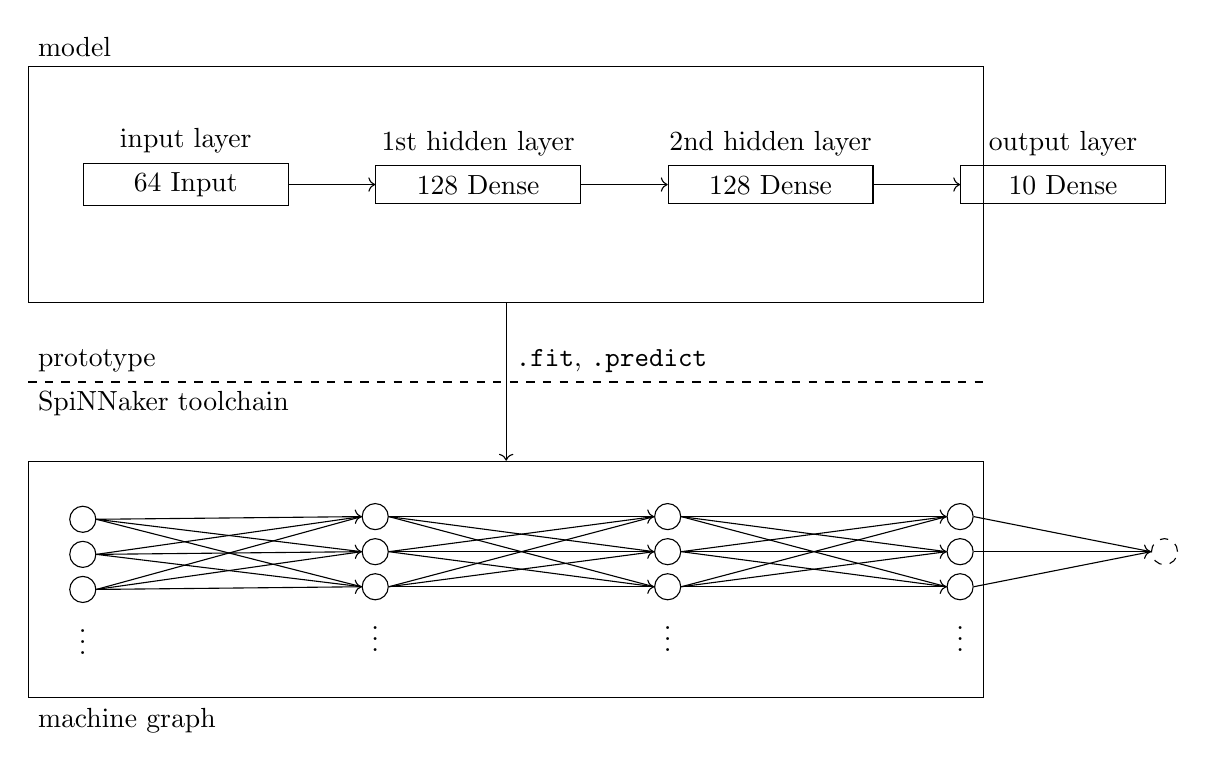
\begin{tikzpicture}[
      elem/.style={rectangle, draw},
      dot/.style={circle, draw},
      layer/.style={minimum width=2.6cm},
      container/.style={minimum width=\linewidth,
                         minimum height=3cm}
    ]
      \node[elem, container]
        at (0, 0) (model) {};
      \node[above right] at (model.north west) {model};

      \node[elem, layer, label=input layer]
        (layer_input) at ($(model.west) + (2, 0)$) {64 Input};
      \node[elem, layer, label=1st hidden layer, right=1.1 of layer_input]
        (layer_hidden1) {128 Dense};
      \node[elem, layer, label=2nd hidden layer, right=1.1 of layer_hidden1]
        (layer_hidden2) {128 Dense};
      \node[elem, layer, label=output layer, right=1.1 of layer_hidden2]
        (layer_output) {10 Dense};

      \draw[->] (layer_input) -- (layer_hidden1);
      \draw[->] (layer_hidden1) -- (layer_hidden2);
      \draw[->] (layer_hidden2) -- (layer_output);


      \draw[dashed] ($(model.south west) - (0, 1)$)
        node[above right] {prototype}
        node[below right] {SpiNNaker toolchain} --
        ($(model.south east) - (0, 1)$);

      \node[elem, container, below=2 of model] (machine_graph) {};
      \node[below right] at (machine_graph.south west)
        {machine graph};

      \node[dot, below=3.8 of layer_input.south west]
        (input0) {};
      \node[dot, below=.1 of input0]
        (input1) {};
      \node[dot, below=.1 of input1]
        (input2) {};
      \node[below=.001 of input2] {\vdots};

      \node[dot, below=3.8 of layer_hidden1.south west]
        (hidden00) {};
      \node[dot, below=.1 of hidden00]
        (hidden01) {};
      \node[dot, below=.1 of hidden01]
        (hidden02) {};
      \node[below=.001 of hidden02] {\vdots};

      \node[dot, below=3.8 of layer_hidden2.south west]
        (hidden10) {};
      \node[dot, below=.1 of hidden10]
        (hidden11) {};
      \node[dot, below=.1 of hidden11]
        (hidden12) {};
      \node[below=.001 of hidden12] {\vdots};

      \node[dot, below=3.8 of layer_output.south west]
        (output0) {};
      \node[dot, below=.1 of output0]
        (output1) {};
      \node[dot, below=.1 of output1]
        (output2) {};
      \node[below=.001 of output2] {\vdots};


      \node[dot, dashed, right=2.25 of output1] (lpg) {};


      \draw[->] (model) -- node[above right]
        {\texttt{.fit}, \texttt{.predict}} (machine_graph);

      \draw[->] (input0.east) -- (hidden00.west);
      \draw (input0.east) -- (hidden01.west);
      \draw (input0.east) -- (hidden02.west);

      \draw (input1.east) -- (hidden00.west);
      \draw[->] (input1.east) -- (hidden01.west);
      \draw (input1.east) -- (hidden02.west);

      \draw (input2.east) -- (hidden00.west);
      \draw (input2.east) -- (hidden01.west);
      \draw[->] (input2.east) -- (hidden02.west);

      \draw[->] (hidden00.east) -- (hidden10.west);
      \draw (hidden00.east) -- (hidden11.west);
      \draw (hidden00.east) -- (hidden12.west);

      \draw (hidden01.east) -- (hidden10.west);
      \draw[->] (hidden01.east) -- (hidden11.west);
      \draw (hidden01.east) -- (hidden12.west);

      \draw (hidden02.east) -- (hidden10.west);
      \draw (hidden02.east) -- (hidden11.west);
      \draw[->] (hidden02.east) -- (hidden12.west);

      \draw[->] (hidden10.east) -- (output0.west);
      \draw (hidden10.east) -- (output1.west);
      \draw (hidden10.east) -- (output2.west);

      \draw (hidden11.east) -- (output0.west);
      \draw[->] (hidden11.east) -- (output1.west);
      \draw (hidden11.east) -- (output2.west);

      \draw (hidden12.east) -- (output0.west);
      \draw (hidden12.east) -- (output1.west);
      \draw[->] (hidden12.east) -- (output2.west);

      \draw (output0.east) -- (lpg.west);
      \draw[->] (output1.east) -- (lpg.west);
      \draw (output2.east) -- (lpg.west);
    \end{tikzpicture}
  \end{center}
  \caption{Illustration of how a machine graph is generated by the
    prototype. The dashed circle represents an auxiliary machine
    vertex, in this case the LPG. This machine graph would be
    generated when the \texttt{predict} method of the model is
    called.}
  \label{fig:spiDNN_arch}
\end{figure} % }}}

The model stores the trainable parameters (the weights of the layers),
which can be accessed via the \texttt{set\_weights} and
\texttt{get\_weights} methods of the model class
(see Listing~\ref{lst:spiDNN_vs_keras}, line 25).
The parameters are generated during the \texttt{add} call by the
added layer, since weights are different for different layer types
and can depend on the preceding layer.
For example, a dense layer (see Section~\ref{subsec:intro_dl})
generates the weight matrix $\mathbf{W}: n \times m$ and the bias
$m$-vector.
$n$ is the number of neurons in the preceding layer, $m$ the number of
neurons of the dense layer.
Convolutional layers do not depend on the previous layer for their
weights.
For example a 1D convolutional layer generates a $3$D array
$\mathbf{W}: \text{\textit{kernel size}} \times channels \times
filters$ and a bias $filters$-vector.
$\mathbf{W}$ are the kernels for each filter (see
Section~\ref{subsec:intro_dl}).
The kernel of a 2D convolutional layer simply has one more spatial
dimension, so the 2D layer would generate a 4D array as weights.
The input layer does not generate any weights.
The format of the weights is again inspired by Keras and enables
seamless interoperability between a SpiNNaker deep learning model and
the subset of the Keras API supported by the prototype
(see Listing~\ref{lst:spiDNN_vs_keras}, line 25).
Having our prototype so closely resemble Keras had the great advantage
of enabling precise integration testing.
We could simply build two equal models, one in Keras and one with our
prototype, and compare their outputs against each other
(see Listing~\ref{lst:spiDNN_vs_keras}, lines 29--36).
The same goes for testing backpropagation, where we could simply train
both models and compare the updated weights
(see Listing~\ref{lst:backprop}).

\begin{figure} % {{{
\begin{lstlisting}[language=Python, caption={Example code comparing
  training with Keras to training with the prototype. The code would
  result in a model (not the machine graph) akin to the one shown in
  Figure~\ref{fig:spiDNN_arch}.}, captionpos=b,
  label=lst:backprop, numbers=left]
import tensorflow as tf
import numpy as np

# prototype library
from spiDNN import Model
from spiDNN.layers import Input, Dense

# random training set
X = np.random.rand(500, 64)
y = np.random.rand(500, 10)

# the keras model
keras_model = tf.keras.Sequential()
keras_model.add(tf.keras.layers.Dense(128, input_shape=(64,)))
keras_model.add(tf.keras.layers.Dense(128, activation=`relu'))
keras_model.add(tf.keras.layer.Dense(10, activation=`softmax'))

# the equivalent model for SpiNNaker
spinn_model = Model()
spinn_model.add(Input(64))
spinn_model.add(Dense(128))
spinn_model.add(Dense(128, activation=`relu'))
spinn_model.add(Dense(10, activation=`softmax'))

# this call ensures both models have the same parameters
model.set_weights(keras_model.get_weights())

# train both models
#
# unlike the prototype, Keras compiles its models, before they can be trained.
# Since the prototype does not offer a optimizer interface yet, it does not
# have a compile method
kmodel.compile(loss=`mean_squared_error',
               optimizer=tf.keras.optimizers.SGD(learning_rate=0.01))
kmodel.fit(X, y, epochs=5, batch_size=32, shuffle=False)

model.fit(
  X, y, loss=`mean_squared_error', epochs=5, batch_size=32, learning_rate=0.01)

error = [x - x_ for x, x_ in zip(model.get_weights(), kmodel.get_weights())]

# difference in weights can happen, due to floating point errors
for e in error:
  assert np.amax(np.absolute(e)) < 0.1
\end{lstlisting}
\end{figure} % }}}

Supported layers are: (\romannumeral 1) input,
(\romannumeral 2) dense and (\romannumeral 3) 1D convolutional layers.
A flatten layer (used for flattening a feature map into a one
dimensional vector so it can be processed by a dense layer) is
implicitly implemented (see Listing~\ref{lst:spiDNN_vs_keras_cnns}).
Besides layers, the prototype supports the following activation
functions:
\begin{itemize}
  \item identity (default when activation unspecified):
    \begin{align}
      f(x) = x
    \end{align}
  \item tanh:
    \begin{align}
      f(x) = tanh(x)
    \end{align}
  \item sigmoid:
    \begin{align}
      f(x) = \frac{1}{1 + \exp(-x)}
    \end{align}
  \item relu (rectified linear unit):
    \begin{align}
      f(x) = max(0, x)
    \end{align}
  \item softmax:
    \begin{align}
      \label{eq:softmax}
      f(x_i) = \frac{\exp(x_i)}{\sum_{j=1}^{N}\exp(x_j)}
    \end{align}
\end{itemize}
The only supported optimizer (algorithm for training the weights) is
gradient descent with a constant learning rate.
Gradient descent is probably the most common optimization algorithm
for deep learning \citep{goodfellow_et_al_2016}.
Supported loss functions, which are optimized, are:
\begin{itemize}
  \item mean squared error:
    \begin{align}
      \label{eq:mse}
      L(y, \hat{y}) = 1/k \sum_{i=1}^k(y_k - \hat{y}_k)^2
    \end{align}

  \item categorical cross-entropy:
    \begin{align}
      L(y, \hat{y}) = - \sum_{i=1}^{k} y_i \log \hat{y}_i
    \end{align}

  \item binary cross-entropy ($y$ and $\hat{y}$ must be scalar):
    \begin{align}
      L(y, \hat{y}) = - y \log \hat{y} + (1 - y) \log(1 - \hat{y})
    \end{align}
\end{itemize}
1D convolutional layers have support for same and valid (default)
padding and they can be strided (see Section~\ref{subsec:intro_dl}
and Listing~\ref{lst:spiDNN_vs_keras_cnns}, lines 30 and 31).

\begin{figure} % {{{
\begin{lstlisting}[language=Python, caption={Example code comparing
  inference with 1D CNNs in Keras to inference with the prototype.},
  captionpos=b, label=lst:spiDNN_vs_keras_cnns, numbers=left]
import tensorflow as tf
import numpy as np

# prototype library
from spiDNN import Model
from spiDNN.layers import Input, Dense, Conv1D

# 64 features, each with 4 channels
input_shape = (64, 4)

# random test set
X = np.random.rand(500, *input_shape)

# the keras model
keras_model = tf.keras.Sequential()
# this layer has 20 filters and a kernel size of 3. Valid padding and a
# stride of 1 are default
keras_model.add(tf.keras.layers.Conv1D(20, 3, input_shape=input_shape))
keras_model.add(tf.keras.layers.Conv1D(5, 3, activation=`relu',
                                       padding=`same', strides=2))
keras_model.add(tf.keras.layers.Flatten())
keras_model.add(tf.keras.layer.Dense(10, activation=`softmax'))

# the equivalent model for SpiNNaker
spinn_model = Model()
spinn_model.add(Input(*input_shape))
spinn_model.add(Conv1D(20, (3,)))
# The feature map of this layer is implicitly flattened,
# because the next layer is a dense layer
spinn_model.add(Conv1D(5, (3,), activation=`relu',
                       padding=`same', stride=2))
spinn_model.add(Dense(10, activation=`softmax'))

# this call ensures both models have the same parameters
model.set_weights(keras_model.get_weights())

# predict the results for the random test set (with random weights)
p_ = kmodel.predict(X)
p = model.predict(X)

error = np.absolute(p - p_)

# difference in prediction can happen, due to floating point errors
assert np.amax(error) < 1e-4
\end{lstlisting}
\end{figure} % }}}

As stated above, a deep learning model is decomposed into neurons
in order to execute it on SpiNNaker.
Neurons are part of the internal APIs of the prototype and not exposed
to the user.
The neuron of a dense layer is a perceptron, which can be seen in
Figure~\ref{fig:perceptron}.
Each neuron of a convolutional layer performs one single convolution
operation with all filters of the layer.
For example, when we look at Figure~\ref{fig:conv_op}, $ax + by + cz$
would be one convolution with one filter.
If the layer has a second filter with a kernel $w, v, u$, the neuron
would produce a second value $aw + bv + cu$.
The input $a, b, c$ stays the same.
A convolutional layer is schematized in Figure~\ref{fig:cnn}.

Figure~\ref{fig:spiDNN_arch} shows how to operate the prototype.
The user defines the sequential deep learning model, like described
above.
Only when the inference or training operations are called is the
model translated into a SpiNNaker machine graph and executed on the
connected machine.
For inference one has to call the \texttt{predict} method of the model
(see Listing~\ref{lst:spiDNN_vs_keras}, line 29)
and for training the \texttt{fit} method
(see Listing~\ref{lst:backprop}, lines 37 and 38).

\begin{algorithm} % {{{
  \caption{: \texttt{predict} method}
  \label{alg:pred}

  \begin{algorithmic}[1]
    \STATE{create extractor layer}
    \STATE{reset layers}
    \STATE{setup SpiNNaker}
    \STATE{initialize machine vertices}
    \STATE{establish forward pass connections}
    \STATE{establish connection between output layer and extractor}
    \STATE{setup live IO}
    \STATE{execute model on SpiNNaker (run forever)}
    \COMMENT{the live IO connection stops the execution}
    \STATE{stop the SpiNNaker machine}
    \STATE{close live IO}
    \RETURN{predictions}
    \COMMENT{predictions collected by live IO}
  \end{algorithmic}
\end{algorithm} % }}}

Algorithm~\ref{alg:pred} shows what happens during the
\texttt{predict} method.
First, an auxiliary layer for the live IO is created, the extractor
layer.
The extractor layer has a single machine vertex, a LPG instance
(see Section~\ref{subsec:spinn_toolchain}) for streaming the
predictions off SpiNNaker, back to the host.
The LPG is also shown as the auxiliary vertex in
Figure~\ref{fig:spiDNN_arch}.
The first layer---which must always be an input layer---handles
streaming the data onto the machine.
Neurons of a input layer are simple wrappers around the RIPTMCS
machine vertices provided by the SpiNNaker toolchain (see
Section~\ref{subsec:spinn_toolchain}).

The layer interface specifies a \texttt{reset} method, which is
called for each layer in Algorithm~\ref{alg:pred}, line 2.
This method resets the neurons of a layer (simply deletes them).
If, for example, the model was trained before the call to the
\texttt{predict} method---probably the most common workflow in deep
learning---the neurons from the training graph would still exist.
Beyond the training these neurons are meaningless, because they were
part of a different run on SpiNNaker and must be deleted (when the
toolchain is reset it deletes its machine graph instance, but the
vertex objects remain).
They could be deleted right before the \texttt{fit} or
\texttt{predict} method exits, but for unit testing it is convenient
to still have the neurons beyond a run on SpiNNaker.

After the machine and the SpiNNaker toolchain are set up, the
machine vertices (neurons) are initialized
(see Algorithm~\ref{alg:pred}, line 4).
The layer interface always sits between the model and the neurons.
The model only ever calls methods of the layers.
This is a design pattern in software engineering called the layered
pattern (not to be confused with the layers provided by our
prototype) \citep{morlion_2018}.
This design pattern is a common way to abstract---e.g.\ TCP/IP or the
OSI model \citep{tanenbaum_et_al_2013}---and keeps code complexity
down, makes ownership clear and helps writing well-defined interfaces.
For the initialization of the neurons, the layer interface provides
a method \texttt{init\_neurons}.
This method generates the neurons, which are stored in the
\texttt{neurons} property of each layer (a Python list).
Furthermore, the \texttt{init\_neurons} method adds the neurons to
the machine graph of the SpiNNaker toolchain.

After the neurons are created and initialized, the connections for
the forward pass are generated (see Algorithm~\ref{alg:pred}, lines 5
and 6).
The layer interface offers the \texttt{connect\_incoming} and
\texttt{connect\_outgoing} functions for this.
Incoming and outgoing refer to the called layer, respectively.
For example, the forward pass is built with calling
\texttt{connect\_incoming} for each hidden layer, the output layer
and the auxiliary layer for extracting the predictions.
Each of these layers is connected with the preceding layer.
All layers except convolutional layers connect each of their neurons
with every neuron of the layer connected with.
Connecting convolutional layers is more complicated, because they
also need to take care of stride and padding.

The last thing to be set up, before execution can start, is the live
IO connection for streaming the observations onto the board and the
predictions off it (see Algorithm~\ref{alg:pred}, line 7).
The communication protocol chosen was the most naive possible
solution, staying true to our development principle (see above).
We called the protocol ping-pong protocol, because the communication
pattern resembles table tennis, the host being one player, the
SpiNNaker machine the other.
The host always sends data onto the board (ping) and receives some
sort of result (pong).
After receiving the pong, another ping is sent by the host or the
execution is stopped when no more data is there to send.
During inference the observations are streamed onto the board as the
ping events.
The deep learning model processes each observation and returns the
predictions of the output layer as the pong event.
Each prediction is collected by the live IO callback function for
receiving data and returned from the \texttt{predict} method
(see Algorithm~\ref{alg:pred}, line 11).

The ping-pong protocol is easy to implement and easy to reason about.
Its main disadvantage is performance.
One can easily see the problem.
Only a single layer is processing an observation at a time.
All other layers wait.
This is a huge waste of time, especially for very deep model
architectures.
A possible solution to this problem is discussed in
Section~\ref{sec:discussion}.

As stated above, weights are actually owned by the model, not
the layer objects.
The weights are directly injected into the neurons during their
generation and initialization.
Conceptually, a perceptron (neuron of a dense layer) owns the weights
associated with its incoming connections.
The filters of the convolutional layers are simply shared between
all neurons of the layer, so each neuron has a copy.

The received packets have to be matched somehow to the weights
the payload of the packet is multiplied by.
All packets sent by the different components of the prototype are
with payload, so 72 bit big.
Each packet consists of a control byte and two words, key and payload
(see Section~\ref{subsec:spinn_toolchain}).
Each neuron knows how many neurons in the previous layer it is
connected to and knows their keys within a certain partition.
The simple MLP shown in Figure~\ref{fig:spiDNN_arch} only has a
single partition---the ``forward'' partition.\footnote{%
  Not actually one
  partition, but lots of outgoing edge partitions with the same
  identifier (see Section~\ref{subsec:spinn_toolchain}).
  Below, a partition will always refer to a set of outgoing edge
  partitions with the same identifier.}
During data generation (see Section~\ref{subsec:spinn_toolchain})
the data structured generated by the SpiNNaker toolchain can be
queried and the machine graph traversed in order to find out the
corresponding routing keys.
The routing keys of the outgoing edge partitions of the neurons
from the previous layer are collected.
The keys are guaranteed to be consecutive.
For example, the first neuron of the input layer of the MLP from
Figure~\ref{fig:spiDNN_arch} (64 neurons big) would have zero as its
key.
The second neuron one.
The first neuron of the first hidden layer would have 64 as key and so
forth.
How we changed the key allocation process to make this guarantee will
be discussed below.

After having collected the keys of the neurons from the previous
layer, the \textit{minimum key} is determined and passed as argument
to the machine vertex running on SpiNNaker.
The weights of the neuron are also passed as an argument to the
machine vertex.
The weights are a simple array of floats.
Now if a packet is received, the weight corresponding to the
connection is simply determined by indexing the weight array with the
index being the key of the received packet minus the minimum key.
The same procedure works for the backward pass as well.
For convolutional neurons it is somewhat more complex, because they
receive multiple channels from their preceding neurons.
The index is therefore determined with an additional array of channel
counters---for each connection a channel counter is created.
A channel counter is incremented each time a value is received from
its corresponding connection.
The channel counter is then additionally used to determine the correct
index of the weight the payload of the packet must be multiplied with.

\begin{algorithm} % {{{
  \caption{: \texttt{receive\_forward}(key, payload) event of a
    perceptron machine vertex}
  \label{alg:receive_forward}

  \begin{algorithmic}[1]
    \STATE{index := key - minimum key}
    \STATE{signals[index] := payload}
    \STATE{receive counter += 1}
  \end{algorithmic}
\end{algorithm} % }}}

Algorithm~\ref{alg:receive_forward} shows the receive event of a
perceptron machine vertex.
Unlike stated above, the payload is stored in an array called
``signals'',
instead of multiplying it directly with its corresponding weight and
summing it up in the perceptron's potential
(see Algorithm~\ref{alg:update}, lines 2--6).
If only inference is done with the deep learning model, this could
be optimized to save precious memory.
Unfortunately, the received signals must be stored for computing the
gradients during the backward pass.
To keep development simple, plain machine vertices for inference and
their trainable counterparts were kept as close to each other as
possible.
Another point in favor of storing the signals, rather than processing
them directly in the receive event, is the fact that SpiNNaker
supports floats only in software and floating point operations are
therefore expensive (they take a lot of cycles)
\citep{furber_et_al_2020}.
Receive events must be processed as fast as possible to keep pressure
off the router, which blocks until the packet is received.
Blocking the router causes back-pressure, which leads to packet loss
(discussed in Section~\ref{subsec:problems}).

\begin{algorithm} % {{{
  \caption{: \texttt{update}() event of a perceptron machine vertex}
  \label{alg:update}

  \begin{algorithmic}[1]
    \IF {receive counter == N}
      \STATE{potential := 0}
      \FOR{(i = 0; i < N; i++)}
        \STATE{potential += signals[i] $\cdot$ weights[i]}
      \ENDFOR
      \STATE{potential += weights[N]}
      \COMMENT{add the bias}
      \STATE{potential := $g$(potential)}
      \COMMENT{apply activation function}
      \STATE{send(forward key, potential)}
      \COMMENT{send potential to next layer}
      \STATE{receive counter := 0}
    \ENDIF
  \end{algorithmic}
\end{algorithm} % }}}

The prototype must support multiple partitions.
For basic inference---without a softmax layer (see below)---it is only
one partition, as stated above.
For the backward pass during training on the other hand, neurons are
not only connected to the neurons of the succeeding layer, but also
to the ones of the preceding layer.
If these backward connections were also part of the ``forward''
outgoing edge partition of the neuron, the potential would reach the
neurons in the preceding layer as well.
In the other direction, the error passed backwards would reach the
neurons in the succeeding layer.
It would be hard to determine if a packet is a potential (meant to
be sent forward) or an error (meant to be sent backward).
Furthermore, this would mean that a lot of MC packets would simply
be dropped by the receiving vertex, because only one set of neurons
handles potentials, while the other only handles errors.
This would put unnecessary strain onto the communication fabric.

Not only does the backward pass needs its own partition, there is
also an activation function which behaves differently to the other
activation functions implemented.
The activation function is the softmax activation function
(see Equation~\ref{eq:softmax}).
Softmax depends on the output of the other neurons of the same layer,
producing a normalized version of the potential.
Softmax is a common activation function for the output layer, making
the output a probability distribution over the $K$ output neurons
\citep{goodfellow_et_al_2016}.

The first implementation of the machine vertices handled softmax
in the next layer or on the host, if the output layer had softmax as
activation function.
Most certainly faster than the current version, it led to awkward
code with more branches.
The amount of overhead in the code and the fact that information
of one layer (its activation function) has to be shared with another
layer was deemed too complex at this stage of the prototype.
The softmax activation function was implemented early in the
development process, when we tried to avoid code complexity at all
cost.
The current version of the prototype handles softmax via an
intra-layer partition, the ``softmax'' partition.
The neurons of a softmax layer are fully connected.
Instead of passing the potential forward (see
Algorithm~\ref{alg:update}, line 8) it is passed sideways to all
neurons in the same layer.
The potentials received on the connections of the softmax partition
are summed in a variable ``denominator''.
When all packets from one pass on the softmax partition are received
(all potentials from the neurons in the same layer), the potential of
the neuron is divided through the denominator and passed forward to
the neurons of the next layer (or the host, respectively).

When we first made the change to add a second partition (softmax
was implemented before backpropagation) we realized that the
SpiNNaker toolchain does allocate its keys per machine vertex.
For example, if we assume the first hidden layer of the deep learning
model in Figure~\ref{fig:spiDNN_arch} to have softmax as its
activation function, the keys for the two partitions of the first
neuron would be 64 (forward partition) and 65 (softmax partition).
The problem with this is that we need our partitions to be
consecutive (see above).
Luckily the toolchain provides a way to override the default key
allocator.

We have overridden the default key allocator with a first-touch
global partition key allocator.
Every time a directed edge is added to the machine graph (e.g.\ as
is done in Algorithm~\ref{alg:pred}, lines 5 and 6) it is mapped to
its place in the key space, such that partitions continue to be
consecutive (global partition over the outgoing edge partitions of
each neuron).
First-touch has two meanings.
On the one hand it means that the first partition will have the lower
keys in the key space.
On the other hand the source neuron of the directed edge added will
have the next biggest key of that partition.
This way we guarantee that, if the connections from the first neuron
of a layer are created before those of the second neuron, the second
neuron will have the key of the first neuron plus one.

The intra-layer connections for the softmax partition are established
during initialization of the neurons (see Algorithm~\ref{alg:pred},
line 4).
This means they are touched by the toolchain prior to the connections
of the forward partition (see Algorithm~\ref{alg:pred}, lines 5 and
6).
If we look at our example from above, where the first hidden layer
of the deep learning model shown in Figure~\ref{fig:spiDNN_arch} has
softmax as its activation function, the keys of the softmax partition
would range from 0 to 127, inclusively (one key per neuron in the
first hidden layer).
The forward keys for the input layer would be 128 to 191, the
forward keys for the first hidden layer would be 192 to 319 and so
forth.
Our first-touch global partition key allocator scales up to an
arbitrary amount of partitions (partitions are obviously bound by the
key space being $2^{32}$ items big), so it is no problem to handle all
four partitions of the prototype:
(\romannumeral 1) the forward partition, (\romannumeral 2) the
softmax partition, (\romannumeral 3) the backward partition and
(\romannumeral 4) the previously unmentioned ``kernel update''
partition.
The kernel update partition works the same way as the softmax
partition.
It is an intra-layer partition to update the filters of a
convolutional layer during the backward pass, since the weights of
the convolutional layer are shared between its neurons
(see Section~\ref{subsec:intro_dl}).

After implementation of the forward pass and the activation functions,
the backward pass was implemented, enabling training a MLP.
The forward pass of trainable neurons works the same with plain
inference neurons, thanks to our development choices (see above).
Training a deep learning model on SpiNNaker is done via the
\texttt{fit} method.
The method takes a training set and its labels as two input
parameters.
Furthermore, one has to define the parameters of the training session.
These parameters are: (\romannumeral 1) the loss function to be
optimized, (\romannumeral 2) the number of iterations over the whole
training set (the epochs), (\romannumeral 3) the batch size for
gradient descent and (\romannumeral 4) the learning rate
(see Section~\ref{subsec:intro_dl}).
The parameters of the training session are passed to the trainable
neurons on the board.
The training set and its labels are streamed onto the board, same as
inference (without the labels).

The structure of the machine graph for a trainable deep learning
model is more complicated than that of simple inference models.
Not only due to the added backward connections, but also the
auxiliary layers are more complex.
First, besides the training data, the labels have to be streamed onto
the board as well.
This is simply done by adding another input layer to the layer
representation of the model.
The labels are needed to compute the loss.
In order to compute the loss, another layer type was implemented,
the loss layer.
An instance of a loss layer is connected to the output layer and the
label input layer.
The loss layer only has a single neuron which computes the loss,
based on the outputs and the labels, and passes its derivatives
backwards to the neurons of the output layer.
The overall loss is also streamed off the board.
The overall loss is displayed to the user in the console, together
with a progress bar.
The input layer has no parameters.
Therefore it can be excluded in the backward pass.
The first hidden layer is connected---backwards---to the LPG used
for streaming data off of SpiNNaker.
Its outputs are used as the pong event.
Once the first hidden layer has computed its gradients the backward
pass is complete and the next forward pass can begin, so the next
example is streamed onto the board.
All the other layers are connected backwards to their preceding
layers.

\begin{algorithm} % {{{
  \caption{: high-level overview of training a deep learning model on
    SpiNNaker}
  \label{alg:backprop}

  \begin{algorithmic}[1]
    \FOR{1,\dots,epochs}
      \FOR{$\mathbf{x}_i \in \mathbf{X}, i=1,\dots,|\mathbf{X}|$}
        \STATE{forward pass $\mathbf{x}_i$}
        \STATE{compute loss}
        \STATE{pass error backwards and compute gradients}
        \IF{($i \mod$ batch size) == 0 || epoch complete}
          \STATE{update weights with (\ref{eq:sgd})}
        \ENDIF
        \IF{last epoch complete}
          \STATE{write weights back to SDRAM}
        \ENDIF
      \ENDFOR
    \ENDFOR
  \end{algorithmic}
\end{algorithm} % }}}

Algorithm~\ref{alg:backprop} gives an overview of how a deep
learning model is trained on SpiNNaker.
The prototype only supports streaming each example individually.
The observation $\mathbf{x}_i$ is passed through the model and the
loss is computed based on the outputs and the labels by the loss layer
(see Algorithm~\ref{alg:backprop}, lines 3 and 4).
For example, let the loss function be mean squared error
(see Equation~\ref{eq:mse}).
The loss is partially derived for each output neuron.
The output of the $i$th neuron is computed as
$\hat{y}_i = g(h(f^{(l-1)}))$, $g$ being the activation function,
$h(\mathbf{x}) = \mathbf{x} \cdot \mathbf{w} + b$.
The partial derivatives in this case are given by:
\begin{align}
  \frac{\delta L}{\delta \hat{y}_i} = 2(\hat{y}_i - y_i).
\end{align}
$\delta L / \delta \hat{y}_i$ is passed backwards to the $i$th neuron
of the output layer and the backward pass begins (see
Algorithm~\ref{alg:backprop}, line 5).
The $i$th output neuron then applies the chain rule in order to
compute its gradients and the error that is passed backwards to each
neuron of the preceding layer (see Equation~\ref{eq:chain_rule}).
$\delta L / \delta \hat{y}_i$ is multiplied with
$\delta \hat{y}_i / \delta h$ (the derivative of the activation
function) to get the \textit{neuron error}.
In order to update the weights, the neuron error is multiplied by the
partial derivation of $h$ to each weight of $\mathbf{w}$:
$\delta h / \delta w_j = f^{(l - 1)}_j$.
The same is done for the bias: $\delta h / \delta b = 1$.

The error passed backwards to the $j$th neuron of the previous layer
is given as the neuron error multiplied by the derivation of the
signal received by the $j$th neuron:
$\delta h / \delta f^{(l-1)}_j = w_j$.
The $j$th neuron of layer $f^{(l-1)}$ sums its total error over all
errors received from the neurons of the succeeding layer.
This process is continued until the neurons of the first hidden layer
have computed their gradients and passed their errors backwards as
the pong event to the host.
The host knows the backward pass is complete and the next
forward pass begins.

Once a batch of backward passes is complete or the epoch has
finished---in the case that the training set size is not divisible by
the batch size---the weights of each neuron of the deep learning model
are updated with
Equation~\ref{eq:sgd}---the sum over the gradients computed in each
backward pass multiplied by the learning rate
(see Algorithm~\ref{alg:backprop}, lines 6--8).
Lastly, the updated weights have to be extracted from the SpiNNaker
machine again, back to the host.
As stated above, the weights are passed onto the machine during the
data generation phase of the SpiNNaker toolchain and are stored in
SDRAM.
Because SDRAM is slow, the weights are copied into DTCM (see
Section~\ref{subsec:intro_spinn}).
The fast and private DTCM memory of each SpiNNaker core can not be
accessed from anywhere but the core itself.
Therefore the updated weights must be written back to the parameter
region in SDRAM, where the host can access them.
This is a very slow operation and is only done after the last
example of the whole training session has been processed
(see Algorithm~\ref{alg:backprop}, lines 9--11).
A constant latency of two seconds has been added to the host.
The host sleeps for two seconds before it extracts the weights from
the machine, to make sure the updated weights are all successfully
copied back to SDRAM.

Last phase of the implementation was spend with implementing 1D
convolutional layers.
Convolutional layers were determined---during the research and planing
phase---to be the hardest part of the implementation.
This turned out to be true, but not for the expected reasons.
We thought that the their general approach to multiple channels and
filters would lead to a complicated implementation.
Rather than having troubles with mapping messages to weights and
updating the kernel, the mapping of a convolutional layer onto neurons
turned out to be awkward and much time was spend on getting padding
and strides right, which were both estimated to be quick and easy to
implement.

In the end, padding and strides turned out to be easy to implement,
once the correct formula was found.
Unfortunately mistakes were made during development, mostly with
calculating offsets for padded neurons, when padding was set to
``same'' (see Section~\ref{subsec:intro_dl}).
Instead of wasting precious resources by creating more neurons in
the preceding layer, which only ever send zero as signal, variables
for upper and lower offsets were calculated for each neuron.
For example, the left-most neuron of the layer shown in
Figure~\ref{fig:padding} has a lower offset of one, whereas the
right-most neuron has an upper offset of one.
An offset of one means, that the neuron does not receive
from \textit{kernel size} many neurons from the previous layer, but
from \textit{kernel size} minus offset many neurons.
For the left-most neuron with a lower offset of one, this means that
its minimum key (see above) does not match to the first
value of each kernel, but to the second.
For the right-most neuron with an upper offset this simply means the
counter which indicated that the forward pass has completed
(see Algorithm~\ref{alg:pred}, line 1) must incorporate the fact
that one neuron from the previous layer is missing (same goes for
lower padding).

Multichannel input and multi-filter output turned out to be
straight-forward to implement.
Simply sending the output of each filter in succession turned out to
be no problem.
On the receiving side a simple counter per neuron was created
(see above).
Flattening a convolutional layer turned out to be no problem as well.
Flattening means that the filter-dimension of the feature map is
reduced, so instead of producing a matrix (in the case of 1D
convolution), the layer actually produces a vector.
This is needed in order to connect a convolutional layer to a dense
layer, because perceptrons cannot handle multichannel inputs.
The 1D convolutional layer of the prototype were flattened by
utilizing the SpiNNaker toolchain.
The toolchain provides the ability to give one outgoing edge partition
multiple keys.
In this case each outgoing edge partition between the neurons of the
convolutional layer and the dense layer in the forward direction has
$filters$ many keys.
Every filter sends with its own key.
This gives the illusion to the dense layer, that it actually is
connected to $filters \cdot n\_neurons$ many neurons in the previous
layer.
In truth it is only connected to $n\_neurons$ many neurons in the
previous layer and each one sends $filters$ many times.

Backpropagation for convolutional layers is more complex than it is
for simple dense layers, for two reasons: (\romannumeral 1) each
filter produces an error which has to be passed backwards and
(\romannumeral 2) weights are shared between the neurons of a
convolutional layer.
Handling backpropagation for convolutional layers have led to the
most complex code of the prototype.

Having to deal with multiple filters in the succeeding layer, which
all produce an error which has to be passed backwards, makes it more
difficult to match between received packets (in the backward
direction) and the filter of the receiving neuron which generated the
error.
Again the problem was solved with counters.
Unfortunately the receiving event for the backward pass in our
implementation has become very complex and computationally too
expensive.
As stated above, the router blocks until a packet is received
(the receive event callback finished).
If the receive event callback takes a long time, the router will be
blocked longer, which will lead to back-pressure on the communication
fabric.
Back-pressure will lead to dropped packets (discussed in
Section~\ref{subsec:problems}).

Shared weights are implemented like the softmax activation function,
with a fully-connected intra-layer partition, the kernel update
partition (see above).
Once the backward pass is complete, the gradients are send to the
other neurons of the layer and simply summed up by each neuron.
Afterwards the gradients are the same for each neuron.
Once the gradients are shared, the errors are passed backwards.

% }}}


\subsection{Problems} % {{{
\label{subsec:problems}

This section describes the mistakes made during
development and the problems encountered.
The only real problem encountered during development was time.
We had the ambitious goal of implementing ResNet-50, a
state-of-the-art deep learning model, on SpiNNaker.
SpiNNaker is a novel neuromorphic computer architecture.
Without prior programming experience on SpiNNaker and with limited
domain knowledge of deep learning, the effort such an endeavor would
take was underestimated.
Without complications, the work plan developed during the research and
planning phase, would have sufficed.
In retrospect it was a naive assumption, that we would not encounter
complications with the power of stalling implementation progress
and this project has been another example of Hofstadter's Law
(see Section~\ref{sec:intro}).
In the end, minor deviations from the work plan added up and time
pressure ensued.
Besides the minor deviations, a major problem with the prototype was
discovered, which we were unable to fix.
This problem has been mentioned in Section~\ref{subsec:SpiDNN_arch}
before and concerns dropped packets.

The minor deviations encountered during the development process
(listed in chronological order) were:

\begin{enumerate}
  \item A bug in the LPG (see Section~\ref{subsec:spinn_toolchain})
  \item Interface changes made to the RIPTMCS during development (see
    Section~\ref{subsec:spinn_toolchain})
  \item A bug discovered during the key generation process for more
    than one key (as is the case for flattened convolutional layers,
    see Section~\ref{subsec:SpiDNN_arch})
  \item Problems with sockets when trying to establish a second live
    IO session (e.g.\ when calling \texttt{predict} after
    \texttt{fit})
  \item Underestimation of the difficulties of implementing strides
    and ``same'' padding for convolutional layers
\end{enumerate}

The first problem encountered was a bug in the LPG.
Between the research and planning phase and the dissertation phase
there was another phase of this project planned.
This phase's goal was familiarization with the SpiNNaker programming
model.
During this phase an example program implementing Conway's game of
life \citep{gardener_1970, furber_et_al_2020} was changed to make it
work with live IO.
The original code can be found at \citet{spinnaker_2020b}.
The implementation using live IO can be found at
\citet{fassbender_2020}.
The original version saves the state of each cell (machine vertex)
on the SpiNNaker machine and extracts the data once the execution is
finished \citep{furber_et_al_2020, spinnaker_2020b}.

We changed the program such that each cell streams its state off the
board.
This did not work once the number of cells exceeded
a certain threshold.
No packets were received by the \texttt{LiveEventConnection}
(see Section~\ref{subsec:spinn_toolchain}) and the router on the
chip with the LPG showed strange warnings of dropped packets.
These warnings were strange because the amount of dropped packets
reported far exceeded the total amount of packets sent during the
whole execution.
SpiNNaker has no memory protection (no segmentation faults when
trying to access memory not owned by the accessing machine vertex).
Any machine vertex can override data owned by other vertices in SDRAM
and we correctly thought that the LPG was writing to memory owned by
the router.
After reducing the code of the LPG, we could determine strange
behavior in the buffer that stores received packets for sending them
to the host.
Once the LPG has sent its first EIEIO message to the host
(see Section~\ref{subsec:SpiDNN_arch}) the buffer showed that it was
full, even though it did not contain packets anymore.
While we could isolate the problem to the generation and sending
process of the EIEIO message, we could not find the bug in there
and had to rely on the SpiNNaker core team to find the bug and fix it.

Finding and fixing this bug took away approximately one week
(the first) of the dissertation phase and the live IO version of
Conway's game of live was not yet finished.
While the states were now streamed off SpiNNaker, the initial
states were not yet streamed onto the machine (a vital part of the
prototype which we had to familiarize ourselves with).
Further interfaces and mechanisms we had to learn were how to
tell SpiNNaker to run forever (see Algorithm~\ref{alg:pred}, line 8)
and how to stop it from the live IO callbacks.
Finishing the implementation of Conway's game of life took another
half week of the dissertation phase.
The issue, a description and a link to the solution can be found at
\citep{fassbender_2020a}.

The interface changes made for the next release of the toolchain
were easily fixable.
The SpiNNaker core team removed the direct support for RIPTMCS
in a machine graph.
Only a single parameter was changed in order to restore the direct
support again (instead of having to use constructs only used in
application graphs).
The change made to the toolchain can be found at
\citet{fassbender_2020b}.

The same goes for the bug discovered during the key allocation
process, once an outgoing edge partition has more than one key,
as is the case with flattened convolutional layers (see
Section~\ref{subsec:SpiDNN_arch}).
For example, a flattened convolutional layer has five filters.
Each neuron therefore has five keys.
The allocation process of the toolchain was overridden by providing
a constraint that tells the toolchain which key to allocate
(a fixed key constraint).
For the flattened layer, five fixed key constraints were passed to
the toolchain, which should return a list with five keys (unsigned
integers).
Let the first neuron of the convolutional layer have the constraints
for keys one to five.
What the toolchain returned was: \texttt{[1, 5, 0, 0, 0]}.
As it turned out, the keys are put into a pre-allocated numpy
array \citep{van_der_walt_2011} of size five.
The constraints are iterated.
A fixed key constraint can return multiple keys, depending on its
mask \citep{furber_et_al_2020}.
We only ever used \texttt{0xFFFFFFFF} as mask, which, in combination
with the fixed key, will only return the fixed key.
So for each iterated constraint, an offset is calculated, depending
on how many keys it has generated.
Unfortunately it was forgotten to sum the offsets up.
The first key (one) generates an offset of one.
The next key (two) is written to the numpy array at the index of
the offset, so to index one.
The second constraint generates an offset of one again.
But instead of adding it to the previous offset, the previous offset
is overwritten.
The offset stays one.
Therefore the third constraint (key is three) is written again to
index one, overwriting the key two.
This continues all the way to five.
Adding two lines that add up the offset instead of overwriting it
solved the problem.
The solution can be found at \citet{fassbender_2020c}.
Both, the interface change and the bug together, were solved in
a single day.

An issue during testing was the
fact that we were unable to get a second live IO session running in
the same Python script, after the first one was properly closed.
This made it impossible to call \texttt{predict} after \texttt{fit},
which is a necessary feature for a working deep learning library for
SpiNNaker.
Otherwise the user would need to export the updated weights to file
and start a new script which loads the weights, before using the
model for inference.
The problem arises due to a socket not being properly closed, or
rather not properly deallocated by the operating system of the host.
In order to fix this problem we tried to tell the operating system to
reuse the socket.
While this removed the error, it led to inconsistent behavior of the
second live IO session.
With the reused socket, the second live IO session sometimes sent
packets to the machine and sometimes did not.

The fact that we were unable to get a second working live IO session
limited our testing abilities in two ways.
First, we could not \texttt{predict} with a trained model (except by
exporting the updated weights to file first, as described above).
Second, we could never execute the whole test suite, but had to
call each function, from every test script, by hand.
While this has been an inconvenience, the overall time spent trying
out the workaround described above and executing the test
suite by hand has not exceeded a whole working day.
The issue can be found at \citep{fassbender_2020d}.

The four issues discussed above were all dealing with the SpiNNaker
toolchain.
Dealing with these issues took approximately two weeks of time during
the dissertation phase.
The last of the minor deviations does not concern itself with the
toolchain, but has its source in mistakes made during the
implementation of the prototype.
As stated in Section~\ref{subsec:SpiDNN_arch}, the time and effort
it would take to get the stride and padding of a convolutional layer
to work was underestimated.
The problem has two sides: (\romannumeral 1) the time it took to find
the right solution and (\romannumeral 2) how difficult it would be
to integrate strides and padding into the machine vertex.
The former could have been prevented by spending more time
on finding the right formula.
Convolutional layers were implemented after forward and backward pass
of the MLP.
Time---unaccounted for in the work plan---was spent debugging cases,
where padding and offset were computed wrongfully.
Getting the formula for computing the offset for strided convolutional
layers with ``same'' padding right took approximately one week.
The difficulties of having to integrate padding into the machine
vertices have been discussed in Section~\ref{subsec:SpiDNN_arch}
(integrating the offset into the forward pass).
The problem with strides arose during the backward pass, where we
have to match the key a packet is sent with to its correct position,
so the errors arrive at their proper place (where they have actually
happened).
In order to get the matching mechanism right, the stride of the
succeeding layer has to be known.
Sharing information between layers is costly concerning code
complexity, something we have learned early during the development
phase while implementing softmax (see
Section~\ref{subsec:SpiDNN_arch}) and backpropagation for MLPs (see
below).
Backpropagation with convolutional layers has been the most complex
task (and the last) implemented in the prototype and it is the main
cause of the major problem limiting supported size of deep learning
models by the prototype: dropped packets.

While we have discussed the general backpropagation mechanism of the
prototype in Section~\ref{subsec:SpiDNN_arch}, we have not looked at
the communication structure of the backward pass.
The reason for that is, that there were three different
communication structures implemented.
All three trying to somehow avoid dropped packets or, in one case,
to avoid code complexity which made another solution unmaintainable.

The problem of dropped packets has been known since the implementation
of the live IO version of Conway's game of life.
The execution of the game of life stopped with an error, once too many
vertices were used.
The problem is that, while the SpiNNaker communication fabric is great
at handling lots of packets, the supported peak of packets being on
the fabric at the same time is not high.
Too many packets on the fabric at the same time causes back-pressure
and the routers simply drop packets.
Therefore packets must be distributed across time.

The SpiNNaker1 API provides a function to the machine vertex called
\texttt{spin1\_set\_timer\_tick\_\-and\_phase}, which allows the user to
define a timer offset.
The timer offset tells the machine vertex when to start its first
update event.
Without the timer offset, the update events of all vertices on the
machine are called at the same time.
During the update event, a cell of Conway's game of life shares its
state with its neighbors.
A perceptron, during the forward pass, may send its potential during
its update event, depending on whether it has received all signals
from the previous layer (see Algorithm~\ref{alg:update}).
If all vertices send at the same time, the peak number of packets on
the communication fabric is obviously high.
With the timer offset one can distribute the peak across time.

The timer offset is computed based on the placement of the neuron on
the board.
Each core of a SpiNNaker machine is uniquely identifiable by a three
element tuple $(x, y, z)$, where $x$ and $y$ are the spatial position
of a SpiNNaker chip in the 2D torus topology of the machine (see
Section~\ref{subsec:intro_spinn}) and $0 \leq z \leq 17$ is the id of
the core on that chip.
During data generation (see Section~\ref{subsec:spinn_toolchain}),
the neuron gets the information about its placement from the
toolchain.
A maximum timer offset is provided by the prototype.
It is the time between update events, divided by ten.
90 percent of the time between update events leaves enough time
for a machine vertex with the maximum offset to send its packets along
the longest path of the topology and the packet being received before
the receiver's next update event.
The formula for computing the maximum offset is taken from
the implementation of a Poisson spike source neuron from the
SpiNNaker front-end for spiking neural networks
\citep{spinnaker_2020c}.
The maximum offset is divided by the cores per chip is multiplied by
$z$.
This way each neuron on a chip has a different offset.

\begin{figure} % {{{
  \begin{subfigure}{.5\textwidth}
  \begin{center}
	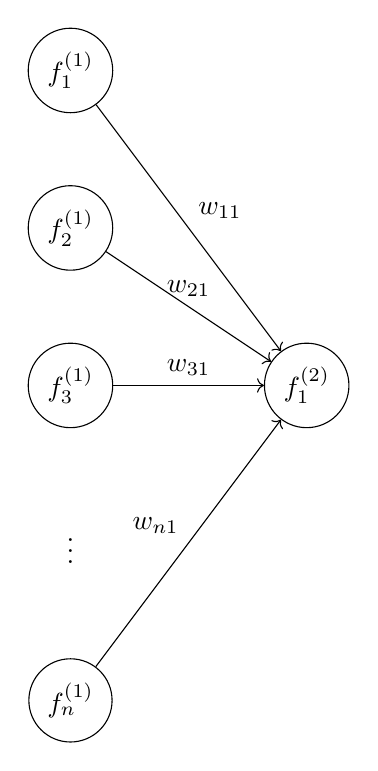
\begin{tikzpicture}[dot/.style={circle,draw}]
		\node at (0,0) [dot] (neuron) {$f^{(2)}_1$};
		\node at (-3,4) [dot] {$f^{(1)}_1$}
			edge[->] node[above right]{$w_{11}$} (neuron);
		\node at (-3,2) [dot] {$f^{(1)}_2$}
			edge[->] node[above]{$w_{21}$} (neuron);
		\node at (-3,0) [dot] {$f^{(1)}_3$}
			edge[->] node[above]{$w_{31}$} (neuron);
		\node at (-3,-4) [dot] {$f^{(1)}_n$}
			edge[->] node[above left]{$w_{n1}$} (neuron);
		\node at (-3,-2) [] {\vdots};
	\end{tikzpicture}
	\end{center}
  \caption{Incoming connections for neuron $f^{(2)}_1$.}
  \label{fig:weights_a}
  \end{subfigure}
  \begin{subfigure}{.5\textwidth}
  \begin{center}
	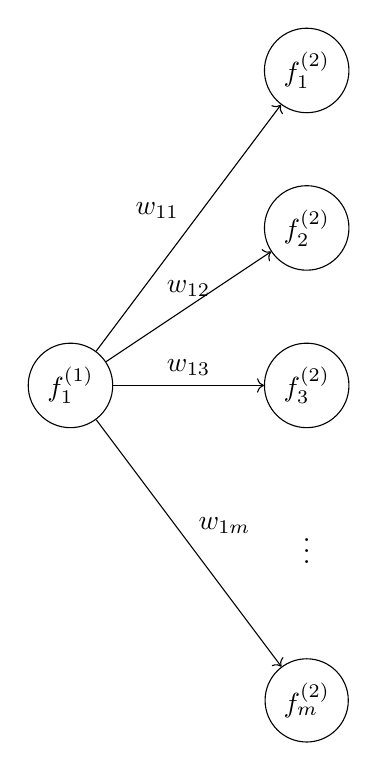
\begin{tikzpicture}[dot/.style={circle,draw}]
		\node at (0,0) [dot] (neuron) {$f^{(1)}_1$};
		\node at (3,4) [dot] {$f^{(2)}_1$}
			edge[<-] node[above left]{$w_{11}$} (neuron);
		\node at (3,2) [dot] {$f^{(2)}_2$}
			edge[<-] node[above]{$w_{12}$} (neuron);
		\node at (3,0) [dot] {$f^{(2)}_3$}
			edge[<-] node[above]{$w_{13}$} (neuron);
		\node at (3,-4) [dot] {$f^{(2)}_m$}
			edge[<-] node[above right]{$w_{1m}$} (neuron);
		\node at (3,-2) [] {\vdots};
	\end{tikzpicture}
	\end{center}
  \caption{Outgoing connections for neuron $f^{(1)}_1$.}
  \label{fig:weights_b}
  \end{subfigure}
\caption {Conceptually, weights can be associated with edges.}
\label{fig:weights}
\end{figure} % }}}

During the forward pass the peak number of packets is low.
Figure~\ref{fig:weights} shows how neurons are connected and how
weights are conceptually bound to the edges.
For example, the output of neuron $f^{(1)}_1$ is multiplied with
weight $w_{11}$, when it is received by neuron $f^{(2)}_1$,
which computes (\ref{eq:perceptron}) during the forward pass.
Weights are owned by the destination neuron of each edge.
So $f^{(2)}_1$ owns all the weights $w_{11},w_{21},\dots,w_{n1}$.
The output of each neuron is passed to all the neurons in the
following layer---if the following layer is a dense layer---or to a
subset of neurons, in the case of a convolutional layer as successor
layer.
Again from the example shown in Figure~\ref{fig:weights}, the output
of $f^{(1)}_1$ would be passed to the neurons $f^{(2)}_1, f^{(2)}_2,
\dots, f^{(2)}_m$.
The forward pass is elegantly solved using a multicast message.
$f^{(1)}_1$ has an outgoing edge partition ``forward'' with all the
edges shown in Figure~\ref{fig:weights_b}.
It sends its output with a single call to the SpiNNaker API to all
the neurons it is connected to and the communication fabric takes care
of multicasting the output to the neurons in the next layer.
Therefore, the peak number of packets on the fabric would be exactly
$n \cdot m$ (only one layer sends at a time, thanks
to the ping-pong protocol presented in
Section~\ref{subsec:SpiDNN_arch}).

For a convolutional layer the peak number of packets is
$n \cdot m \cdot filters / stride$.
Each filter produces a different result
(see Section~\ref{subsec:intro_dl}).
For each filter, one call to the SpiNNaker API is necessary in order
to multicast its output to the next layer.
To reduce the added pressure of having multiple filters, we introduced
a constant latency into the sending loop.
This keeps the peak number of packets lower by spreading the
packets across time, like using the timer offset (see above).

For development we had access to one SpiNN-5 board
(see Section~\ref{subsec:intro_spinn} and
Appendix~\ref{sec:spinn_photos}).
The SpiNN-5 board has 48 chips, which means it has 864 cores.
One core per chip is reserved for the router, so a maximum of 816
cores can be used for neurons.
Extra monitor cores can be enabled to decrease loading time before the
execution starts and for packet re-injection of dropped packets
(see below), which decreases the number of cores per chip down to 15
\citep{furber_et_al_2020}.
Listing~\ref{lst:big_models_inference} shows an excerpt from the test
suite.
Inference with two models, one MLP and one CNN, is tested.
Both models have enough neurons to fill the whole board (816 cores).
Neither one experiences problems with dropped packets.

Backpropagation puts much more pressure onto the communication
fabric.
During backpropagation, neuron $f^{(2)}_1$ in
Figure~\ref{fig:weights_a} computes its neuron error (see
Section~\ref{subsec:SpiDNN_arch}).
In order to get the error that is passed backwards, the neuron error
is multiplied by each weight.
The error passed from $f^{(2)}_1$ to $f^{(1)}_1$ is the neuron error
of $f^{(2)}_1$ multiplied with $w_{11}$.
The error passed to $f^{(1)}_2$ is the neuron error multiplied with
$w_{21}$ and so forth.
The problem is, neuron $f^{(2)}_1$ owns all the weights
$w_{11}, w_{21}, \dots, w_{n1}$.
$f^{(1)}_1$ does not know about $w_{11}$ and cannot access it.
There were three approaches to solving the problem:
(\romannumeral 1) one-to-one backward partitions,
(\romannumeral 2) shared parameters and (\romannumeral 3)
multicasting each error.

The first approach was to compute each error passed backwards
from $f^{(2)}_1$ inside the neuron and send each error successively,
via a one-to-one outgoing edge partition.
This way, $f^{(2)}_1$ would have $n$ outgoing edge partitions, each
with one destination.
In comparison, $f^{(1)}_1$ has one outgoing edge partition in the
forward direction with $n$ destinations.
This approach has one major disadvantage: pressure on the routing
table.
Each outgoing edge partition has one unique key
(see Section~\ref{subsec:spinn_toolchain}).
This way, $m \cdot n$ keys are needed only for layer two shown in
Figure~\ref{fig:weights}, instead of
$m$ keys for all the outgoing edge partitions of the layer in the
forward direction.
Each router has a 1024 word routing table
\citep{navaridas_et_al_2009}.
Even though the SpiNNaker toolchain offers routing table compression
\citep{heathcote_2016}, lots of small partitions will cause too many
entries.
The number of entries does not fit into the routing table, even for
small networks.
It was clear that this approach does not offer a scalable solution
and was abandoned quickly.
It took approximately half a week to develop and test this version of
backpropagation.

Since we knew about the problem of dropped packets, we continued
searching for a solution with minimal packets, rather than the most
naive and easiest to implement.
The next approach represents an unsuccessful trade-off between code
quality and scalability.
Since we did not experience dropped packets during the forward pass on
a MLP filling all the available cores on a SpiNN-5 board (see
Listing~\ref{lst:big_models_inference}), we deemed that sending
$n \cdot m$ packets works well enough (tested with a maximum $n$ of 50
and $m$ of 300, which makes the peak number of packets 15,000).
In order to achieve one call to the SpiNNaker API per neuron for
sending backwards, we introduced shared parameters.
Shared parameters means that $f^{(1)}_1$ now owns and maintains a copy
of $w_{11}, w_{12}, \dots, w_{1m}$, which are owned by the neurons of
layer two.
If the next layer is a convolutional layer, the neurons own a copy of
the whole kernel of the succeeding layer.
$f^{(2)}_1$ only has to send its neuron error backwards.
It reaches every neuron in layer one.
The neurons in layer one compute their error by multiplying the
received neuron error with $w_{i1}$, now that they own a copy of the
weight.
This way the same number of packets are sent forward and backward.
Forward and backward partition between two layers are simply reversed
(outgoing edge partition of $f^{(1)}_1$ in the forward direction has
the $m$ destinations in the succeeding layer, while the outgoing
edge partition of $f^{(2)}_1$ in the backward direction has $n$
destinations in the preceding layer).

As stated in Section~\ref{subsec:SpiDNN_arch}, we early on realized
the code complexity arising from sharing information between layer
objects in the context of the softmax activation function.
Therefore, we tried to avoid breaking the layered design pattern
we chose for the prototype.
Compared to softmax, sharing weights between neurons is a severe
violation of this pattern.
Furthermore, it violated our design philosophy: prototype before you
polish (see Section~\ref{subsec:spinn_toolchain}).

Another negative aspect of sharing parameters is the fact that the
computational effort of the backward pass and the amount of memory
needed for the whole model are doubled.
$w_{11}$ now has to be updated by two different neurons, its
conceptual owner $f^{(2)}_1$ and the neuron which owns a copy
$f^{(1)}_1$.
If $w_{11}$ is only updated by the owner, the error of $f^{(1)}_1$
would be computed wrongly, because the neuron error of $f^{(2)}_1$ is
multiplied by the outdated weight.
Therefore, $f^{(1)}_1$ has to perform gradient descent not only for
the weights it owns, but also for the copies of the weights of the
succeeding layer.
The copied weights and their gradients have to be stored by
$f^{(1)}_1$ as well.
The overall memory needed by the deep learning model (ignoring the
constant memory needed for variables) is doubled.

Sharing parameters was deemed good enough of a compromise between
scalability and code complexity during the backward pass
implementation of the MLP.
We were able to train a model similar to the MLP shown in
Listing~\ref{lst:big_models_inference} to learn XOR
(see Listing~\ref{lst:big_mlp_training}), without dropped packets.
Therefore, we modeled our implementation of 1D convolutional layers
based on shared parameters.
In retrospect, this turned out to be the wrong decision and can be
accounted to the miscalculation of the effort it would take to
implement convolutional layers (see Section~\ref{subsec:SpiDNN_arch}).
The complexity of having to update weights of a convolutional layer
not only intra-layer, but also across layers turned out to be too
complex to implement in the time allocated for this thesis.
Trying to solve the issue arising with padding and strides described
above in addition to a backward pass algorithm for convolutional
layers which turned out to be much higher in complexity than the
backward pass algorithm for dense layers took all the remaining time
intended for implementation and most of the time reserved as a
buffer (three weeks buffer reserved for improving the implementation
and for benchmarking, out of thirteen weeks of dissertation phase).
In the end, we were not able to get the backward pass working for
convolutional layers with shared parameters.

\begin{algorithm} % {{{
  \caption{: Backward pass for the approach of multicasting each
    error}
  \label{alg:multicast_error}

  \begin{algorithmic}[1]
    \STATE{compute neuron error}
    \FOR{$i = 1,\dots,n$}
      \STATE{error $:= \text{neuron error} \cdot w_{ij}$}
      \COMMENT{$j$ is the constant index of the neuron executing this
        algorithm}
      \STATE{send error backwards to all connected neurons in the
        preceding layer}
      \STATE{(optionally) add latency in-between iterations, in order
        to spread the packets in time}
    \ENDFOR
  \end{algorithmic}
\end{algorithm} % }}}

When it became clear that shared parameters are too complex to
implement and maintain, we changed our approach for communication
during the backward pass again, trying to tackle the problem arising
from the complexity of the code.
We chose to compute the error passed backwards inside $f^{(2)}_1$.
This approach is like our first approach, without one-to-one
partitions.
The partition structure stays the same as the structure of the
forward pass and the structure of the shared parameters approach for
the backward pass.
This approach puts massive pressure on the communication fabric.
Algorithm~\ref{alg:multicast_error} shows the backward pass procedure
for communicating the errors backwards.
The problem arises in Algorithm~\ref{alg:multicast_error}, line 4.
For example, if $f^{(2)}_1$ from Figure~\ref{fig:weights} sends the
error intended for $f^{(1)}_1$ backwards, it will reach all $n$
neurons it is connected to from the preceding layer.
The other neurons $f^{(1)}_2, f^{(1)}_3, \dots, f^{(1)}_n$ all receive
a packet and drop it, since it is not their error.
In the second iteration $f^{(1)}_2$ receives the error and all other
neurons drop their multicast packet.
This is continued $n$ times.
The peak number of packets increases from $m \cdot n$ to
$m \cdot n^2$.
Of those $n^2$ packets, $n(n - 1)$ are simply dropped at the receiving
end.
These packets do not serve a purpose in themselves and are only used
to increase a counter, so the receiving neuron knows if the received
error is the one intended for it.
If we look at the MLP from Listing~\ref{lst:big_models_inference},
lines 24--31, it has a 300 neuron layer, followed by a 50 neuron
layer.
A forward pass between these two layers needs 15,000 packets
(see above).
The backward pass from the 50 neuron layer to the 300 neuron layer
multiplies this with a factor of 300.
The peak number of packets increases from 15,000 packets to 4,500,000.
4,485,000 packets are dropped at the receiving end.
Over 99 percent of all packets sent during the backward pass are
unused.

With multicasting errors backwards, we were able to get
backpropagation working for convolutional layer.
Listing~\ref{lst:cnn_known_weights} shows the test we used for
implementing backpropagation.
We computed the gradients by hand, controlled them with the Keras
model and tried to implement the backward pass accordingly.
We were unable to make this test work with shared parameters.
With multicasting errors, we managed to pass the test.
The biggest CNN trained with this approach can be seen in
Listing~\ref{lst:training_cnn}.
Beyond this size, dropped packets stalled the execution.
Even for such a small deep learning model, we experienced exploding
gradients (up to the point where weights turned to NaN)
\citep{brownlee_2019a}, whereas the Keras model used for comparing
did not.
This could have three reasons: (\romannumeral 1) Keras has some
mechanism to avoid exploding gradients the author does not know about,
(\romannumeral 2) floating operations on SpiNNaker are numerically
unstable and (\romannumeral 3) the most likely reason being a bug
in the prototype.

Another major problem of multicasting errors backwards, besides the
number of unused packets straining the communication fabric, is
the amount of time spent by the receive callback.
As stated in Section~\ref{subsec:SpiDNN_arch}, while a packet is
received by a core, the router on that chip blocks.
Therefore, receive callbacks must be fast, to keep the time the router
is blocked down.
Receiving multicasted errors backwards takes time, because the
receiver must find out, if the received packets is intended for
it.
As stated above, this is done by increasing a counter.
For dense layers, receiving backwards is not too complex.
Neurons of a convolutional layer on the other hand spend a lot of
time in their receive callback.
They not only have to increase the counter and see, whether the
packets received is one of its errors.
Also, they have to deal with the extra complexity of having not only
to receive one error from the sending neuron.
They need to receive as many packets from a neuron in the succeeding
layer, as this layer has filters (channels of the succeeding layer),
multiplied by the amount of filters of the succeeding layer.
Therefore, matching received packets takes time, pressuring the
communication fabric even more.
Ironically, in order to match received packets, the neuron needs to
know about the stride of the succeeding layer, so even the less
complex solution compared to shared parameters needs to violate
the layered design pattern.

The SpiNNaker toolchain offers a utility called a packet re-injector
\citep{furber_et_al_2020}.
The re-injector is a machine vertex running on each chip.
It collects dropped packets by the blocked router and stores them.
Later, once the router is not blocked anymore, it re-injects the
packets into the router.
There is only one register in the SpiNNaker hardware for dropped
packets \citep{furber_et_al_2020}.
If a second packet is dropped, before the re-injector can take the
first dropped packet from the register, the first packet will be lost,
without possibility to recover.
Even with the re-injector and increasing the time between update
events from five microseconds to ten, multicasting errors backwards
was not able to scale in a meaningful way.

After trying out multicasting errors backwards, without much success
and seeing its scaling errors in practice, we ran out of time.
We could not solve the problem of dropped packets and were unable to
get the more complex approach to the backward pass---shared
parameters---working.
We were unable to get the prototype to a state where it would have
sufficed for implementing ResNet-50 with it---the model we originally
intended to benchmark our prototype with
(see Section~\ref{subsec:intro_bench}).
The missing features are: (\romannumeral 1) 2D convolutional layers,
(\romannumeral 2) pooling layers and (\romannumeral 3) shortcut
connections (see Section~\ref{subsec:intro_bench}).

% }}}

% }}}


\section{Discussion} % {{{
\label{sec:discussion}

In this section we will discuss further issues with and enhancements
to the prototype.
Besides the problem of not being able to implement a version of the
backward pass which would enable a model on the scale of ResNet-50,
we discovered some issues with our general approach to implementing
deep learning on SpiNNaker and with our hypothesis, that neurons
are a good choice for domain decomposition of a deep learning model
(see Section~\ref{subsec:SpiDNN_arch}).
Untested solutions for the problem with dropped packets are presented,
as is an idea for better domain decomposition, which could solve (or
at least mend) two major issues with the prototype at once:
(\romannumeral 1) a lower peak number of packets and (\romannumeral 2)
the previously undiscussed issue, that decomposing a deep learning
model into neurons implemented as machine vertices on SpiNNaker leads
to resource invariance and therefore to poorer performance.
Performance has not been discussed previously, simply due to the
fact that a working solution must be achieved first, before it can
be made fast.
But since the goal of this thesis is to communicate shortcomings of
our prototype and our hypothesis (see Section~\ref{sec:intro})---so
the next efforts of implementing deep learning on SpiNNaker can build
on the knowledge gained during this work---we have to communicate the
observations made about performance, as well as complexity and
functionality.

We chose neurons as abstractions because we thought them
straightforward to implement.
For perceptrons, this turned out to be correct.
Implementing a convolutional layer based on neurons---where each
neuron does one convolution with all filters of the layer
(see Section~\ref{subsec:SpiDNN_arch})---turned out to be quite
complex.
The major complexity arises during the backward pass and strides and
padding being hard to integrate into the neurons (see above).

Besides not being as straightforward to implement and not as easy to
reason about as was expected, our prototype has another flaw: resource
invariance.
This can be attributed to the early stage this project is in.
The SpiNNaker toolchain offers a way to make neurons more resource
aware, namely application graphs.
Application graphs can combine multiple neurons
into one core, fully utilizing its resources (see
Section~\ref{subsec:spinn_toolchain}).
The problem with application graphs in this context is, that they
cannot handle neurons (atoms for the application graph) which will
not fit into a single core.
For example, the middle layer of one of the last three residual blocks
of ResNet-50 (see Section~\ref{subsec:intro_bench}) performs a
$3 \times 3$ convolution on a feature map with 512 channels and
has 512 filters.
Storing the weights alone takes 9,216 Kb, far exceeding the available
64 Kb of DTCM of a single core (see Section~\ref{subsec:intro_spinn}).
This is another problem which can be added to the missing features
for ResNet-50.
Deep learning neurons can grow very big and it can happen that they
have to be split up.
Conceptually this is solvable by utilizing the SpiNNaker toolchain,
which offers a concept called shared keys, allowing multiple outgoing
edge partitions to have the same key.
This way a receiving neuron would not know that it is receiving from
different cores.

Another example illustrating the resource invariance of neurons as
machine vertices are bottlenecks.
If one would execute a three layer MLP with 10, 1000 and 20 neurons
per layer, the second layer would take 1000 cores, each core having
a tenth of the computational effort compared to the 20 cores taken
by the output layer.
ResNet-50 is another example.
Each time a residual block halves the spatial dimensions of its
input (applies a stride of two, see Section~\ref{subsec:intro_bench}),
it doubles the number of filters \citep{he_et_al_2015}.
This should keep computational cost per layer identical.
For our prototype, the computational effort would simply rise, each
time the filters are doubled.
The layers that are computationally more demanding receive less space
on the board---less resources---than the computationally less
demanding layers.

\begin{figure} % {{{
  \begin{subfigure}{\linewidth} % {{{
    \begin{center}
    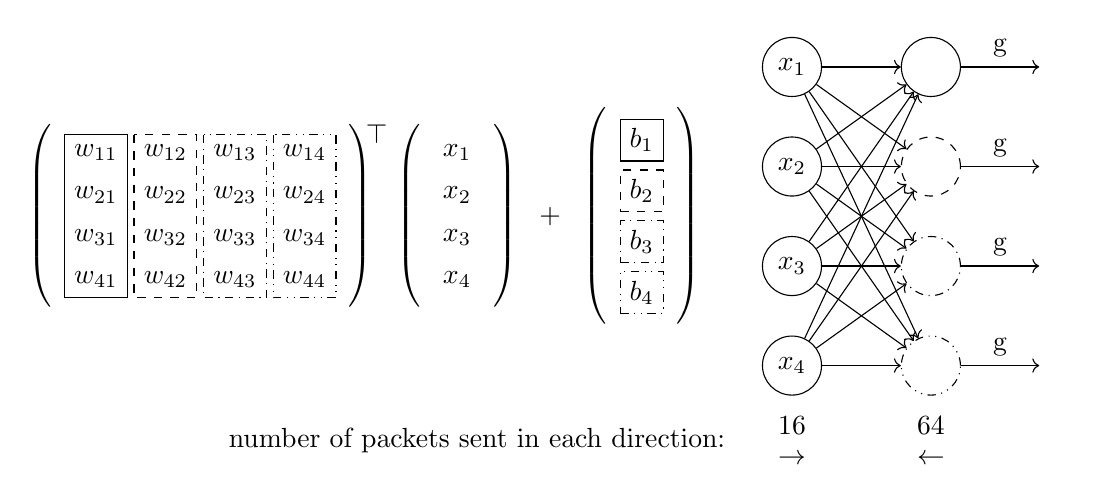
\begin{tikzpicture}[dot/.style={circle,draw, minimum size=.75cm}]
      \matrix[left delimiter=(, right delimiter=), column sep=.1cm, row sep=.1cm] (w) {
        \node (w_11) {$w_{11}$}; & \node (w_12) {$w_{12}$}; & \node (w_13) {$w_{13}$}; & \node (w_14) {$w_{14}$}; \\
        \node (w_21) {$w_{21}$}; & \node (w_22) {$w_{22}$}; & \node (w_23) {$w_{23}$}; & \node (w_24) {$w_{24}$}; \\
        \node (w_31) {$w_{31}$}; & \node (w_32) {$w_{32}$}; & \node (w_33) {$w_{33}$}; & \node (w_34) {$w_{34}$}; \\
        \node (w_41) {$w_{41}$}; & \node (w_42) {$w_{42}$}; & \node (w_43) {$w_{43}$}; & \node (w_44) {$w_{44}$}; \\
      };
      \node at ($(w.north east) + (.4,-.1)$) {$\top$};
      \matrix[right=1 of w, row sep=.1cm, left delimiter=(, right delimiter=)] (x) {
        \node{$x_1$}; \\
        \node{$x_2$}; \\
        \node{$x_3$}; \\
        \node{$x_4$}; \\
      };
      \node[right=.5 of x] (add) {+};
      \matrix[right=.5 of add, row sep=.1cm, left delimiter=(, right delimiter=)] (b) {
        \node[draw]{$b_1$}; \\
        \node[draw, dashed]{$b_2$}; \\
        \node[draw, dash dot]{$b_3$}; \\
        \node[draw, dash dot dot]{$b_4$}; \\
      };

      \matrix[right = 1 of b, column sep=1cm, row sep=.5cm] {
        \node[dot] (x_1) {$x_1$}; & \node[dot] (n_1) {}; & \node (o_1) {}; \\
        \node[dot] (x_2) {$x_2$}; & \node[dot, dashed] (n_2) {}; & \node (o_2) {}; \\
        \node[dot] (x_3) {$x_3$}; & \node[dot, dash dot] (n_3) {}; & \node (o_3) {}; \\
        \node[dot] (x_4) {$x_4$}; & \node[dot, dash dot dot] (n_4) {}; & \node (o_4) {}; \\
      };

      \node[below=1 of x_4.center, label=16] (packets) {$\rightarrow$};
      \node[below=1 of n_4.center, label=64] {$\leftarrow$};
        \node at ($(packets.north) - (4,-.05)$) {number of packets sent in each direction:};

      \draw[->] (x_1) -- (n_1);
      \draw[->] (x_1) -- (n_2);
      \draw[->] (x_1) -- (n_3);
      \draw[->] (x_1) -- (n_4);

      \draw[->] (x_2) -- (n_1);
      \draw[->] (x_2) -- (n_2);
      \draw[->] (x_2) -- (n_3);
      \draw[->] (x_2) -- (n_4);

      \draw[->] (x_3) -- (n_1);
      \draw[->] (x_3) -- (n_2);
      \draw[->] (x_3) -- (n_3);
      \draw[->] (x_3) -- (n_4);

      \draw[->] (x_4) -- (n_1);
      \draw[->] (x_4) -- (n_2);
      \draw[->] (x_4) -- (n_3);
      \draw[->] (x_4) -- (n_4);

      \draw[->] (n_1) -- node[above]{g} (o_1);
      \draw[->] (n_2) -- node[above]{g} (o_2);
      \draw[->] (n_3) -- node[above]{g} (o_3);
      \draw[->] (n_4) -- node[above]{g} (o_4);

      \draw (w_11.north west) |- (w_41.south west) -| (w_11.north east) -- cycle;
      \draw[dashed] (w_12.north west) |- (w_42.south west) -| (w_12.north east) -- cycle;
      \draw[dash dot] (w_13.north west) |- (w_43.south west) -| (w_13.north east) -- cycle;
      \draw[dash dot dot] (w_14.north west) |- (w_44.south west) -| (w_14.north east) -- cycle;
    \end{tikzpicture}
    \end{center}
    \caption{How the computational graph of a dense layer is
      decomposed into neurons.}
    \vspace{1cm}
  \end{subfigure} % }}}
  \begin{subfigure}{\linewidth} % {{{
    \begin{center}
    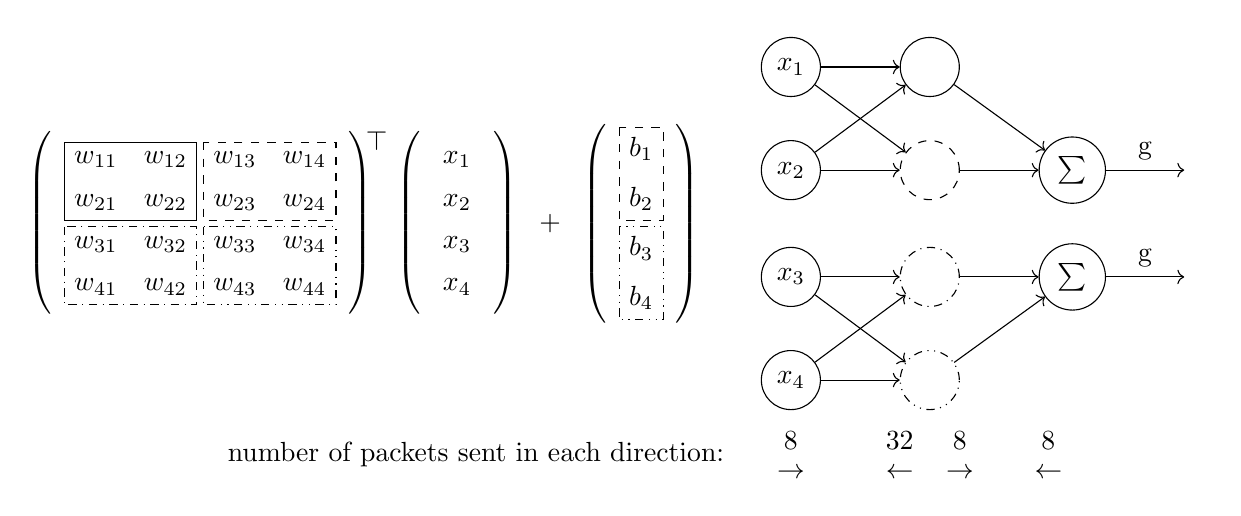
\begin{tikzpicture}[dot/.style={circle,draw, minimum size=.75cm}]
      \matrix[left delimiter=(, right delimiter=), column sep=.1cm, row sep=.1cm] (w) {
        \node (w_11) {$w_{11}$}; & \node (w_12) {$w_{12}$}; & \node (w_13) {$w_{13}$}; & \node (w_14) {$w_{14}$}; \\
        \node (w_21) {$w_{21}$}; & \node (w_22) {$w_{22}$}; & \node (w_23) {$w_{23}$}; & \node (w_24) {$w_{24}$}; \\
        \node (w_31) {$w_{31}$}; & \node (w_32) {$w_{32}$}; & \node (w_33) {$w_{33}$}; & \node (w_34) {$w_{34}$}; \\
        \node (w_41) {$w_{41}$}; & \node (w_42) {$w_{42}$}; & \node (w_43) {$w_{43}$}; & \node (w_44) {$w_{44}$}; \\
      };
      \node at ($(w.north east) + (.4,-.1)$) {$\top$};
      \matrix[right=1 of w, row sep=.1cm, left delimiter=(, right delimiter=)] (x) {
        \node{$x_1$}; \\
        \node{$x_2$}; \\
        \node{$x_3$}; \\
        \node{$x_4$}; \\
      };
      \node[right=.5 of x] (add) {+};
      \matrix[right=.5 of add, row sep=.1cm, left delimiter=(, right delimiter=)] (b) {
        \node (b_1) {$b_1$}; \\
        \node (b_2) {$b_2$}; \\
        \node (b_3) {$b_3$}; \\
        \node (b_4) {$b_4$}; \\
      };

      \matrix[right = 1 of b, column sep=1cm, row sep=.5cm] {
        \node[dot] (x_1) {$x_1$}; & \node[dot] (n_1) {}; & \node (o_1) {}; & \node (oo_1) {}; \\
        \node[dot] (x_2) {$x_2$}; & \node[dot, dashed] (n_2) {}; & \node[dot] (o_2) {$\sum$}; & \node (oo_2) {}; \\
        \node[dot] (x_3) {$x_3$}; & \node[dot, dash dot] (n_3) {}; & \node[dot] (o_3) {$\sum$}; & \node (oo_3) {}; \\
        \node[dot] (x_4) {$x_4$}; & \node[dot, dash dot dot] (n_4) {}; & \node (o_4) {}; & \node (oo_4) {}; \\
      };

      \node[below=1 of x_4.center, label=8] (packets) {$\rightarrow$};
      \node[below=1 of n_4.west, label=32] {$\leftarrow$};
      \node[below=1 of n_4.east, label=8] {$\rightarrow$};
      \node[below=1 of o_4.center, label=8] {$\leftarrow$};
        \node at ($(packets.north) - (4,-.05)$) {number of packets sent in each direction:};

      \draw[->] (x_1) -- (n_1);
      \draw[->] (x_1) -- (n_2);

      \draw[->] (x_2) -- (n_1);
      \draw[->] (x_2) -- (n_2);

      \draw[->] (x_3) -- (n_3);
      \draw[->] (x_3) -- (n_4);

      \draw[->] (x_4) -- (n_3);
      \draw[->] (x_4) -- (n_4);

      \draw[->] (n_1) -- (o_2);
      \draw[->] (n_2) -- (o_2);
      \draw[->] (n_3) -- (o_3);
      \draw[->] (n_4) -- (o_3);

      \draw[->] (o_2) -- node[above]{g} (oo_2);
      \draw[->] (o_3) -- node[above]{g} (oo_3);

      \draw (w_11.north west) |- (w_21.south west) -| (w_12.north east) -- cycle;
      \draw[dashed] (w_13.north west) |- (w_23.south west) -| (w_14.north east) -- cycle;
      \draw[dash dot] (w_31.north west) |- (w_41.south west) -| (w_32.north east) -- cycle;
      \draw[dash dot dot] (w_33.north west) |- (w_43.south west) -| (w_34.north east) -- cycle;

      \draw[dashed] (b_1.north west) |- (b_2.south west) -| (b_1.north east) -- cycle;
      \draw[dash dot dot] (b_3.north west) |- (b_4.south west) -| (b_3.north east) -- cycle;
    \end{tikzpicture}
    \end{center}
    \caption{How the computational graph of a dense layer could
      be decomposed in order to reduce the peak and overall number of
      packets by sparsifying the graph.}
    \vspace{1cm}
  \end{subfigure} % }}}
  \caption{Illustration of how a dense layer could be decomposed
  in order to reduce the peak number of packets. The number of
  packets sent are based on multicasting errors backwards (see
  Section~\ref{subsec:problems}).}
  \label{fig:domain_decomp}
\end{figure} % }}}

% here present better domain decomposition for dense layer

% CNNs pretty much the same but with higher dimensions

%
% SpiNNaker toolchain may remove resource invariance, but proper
% domain decomposition will also mend the problem of dropped packets

% streaming and ping-pong not good (the first for batch norm, the
% other means a lot of waiting neurons, not doing anything

\begin{itemize}
  \item interpreting neurons as domain decomposition over linear algebra
    compute graph
  \item present possible solutions for problems encountered
  \item space used inefficiently (cores and memory) $\rightarrow$ better
    domain decomposition
  \item with this streaming model I have no easy way to do batch
    normalization---implications for vanishing/exploding gradients
    during training
  \item Ping-pong protocol sucks performance wise
  \item optimizations from README
  \item gradients not shared after each pass but only before weight
    update
\end{itemize}


% }}}


\section{Conclusion}
\label{sec:conclusion}

% here the recap

\section{Next Steps}
\label{sec:next_steps}

\begin{itemize}
  \item profiling
  \item cost model
  \item multiple copies of the same network on the same machine
    $\rightarrow$ use all resources available
  \item better domain decomposition (SpiNNaker application graph or
    custom solution (application graph not helpful for neurons which
    become too big))
  \item smart algorithms vs.\ integrating with state-of-the-art libraries
    (investing time in stuff like SLIDE and the one paper by the Austrian
    guys about sparse connections explicitly mentioning SpiNNaker and
    neuromorphic chips or rather work on a trans-/compiler
    that efficiently translates linear algebra operations (like TF,
    PyTorch,\dots) onto SpiNNaker)
  \item integrate into compiler projects like Apache-TVM, XLA, Glow,
   nGraph, etc.
  \item implementing ONNX spec to make it easy for developers to use
    SpiNNaker (develop in PyTorch $\rightarrow$ run on SpiNNaker)
\end{itemize}

\bibliography{library.bib}
\addcontentsline{toc}{section}{References}


\begin{appendices}
\section{Images of the SpiNNaker Hardware}
\label{sec:spinn_photos}

\begin{figure}[H]
  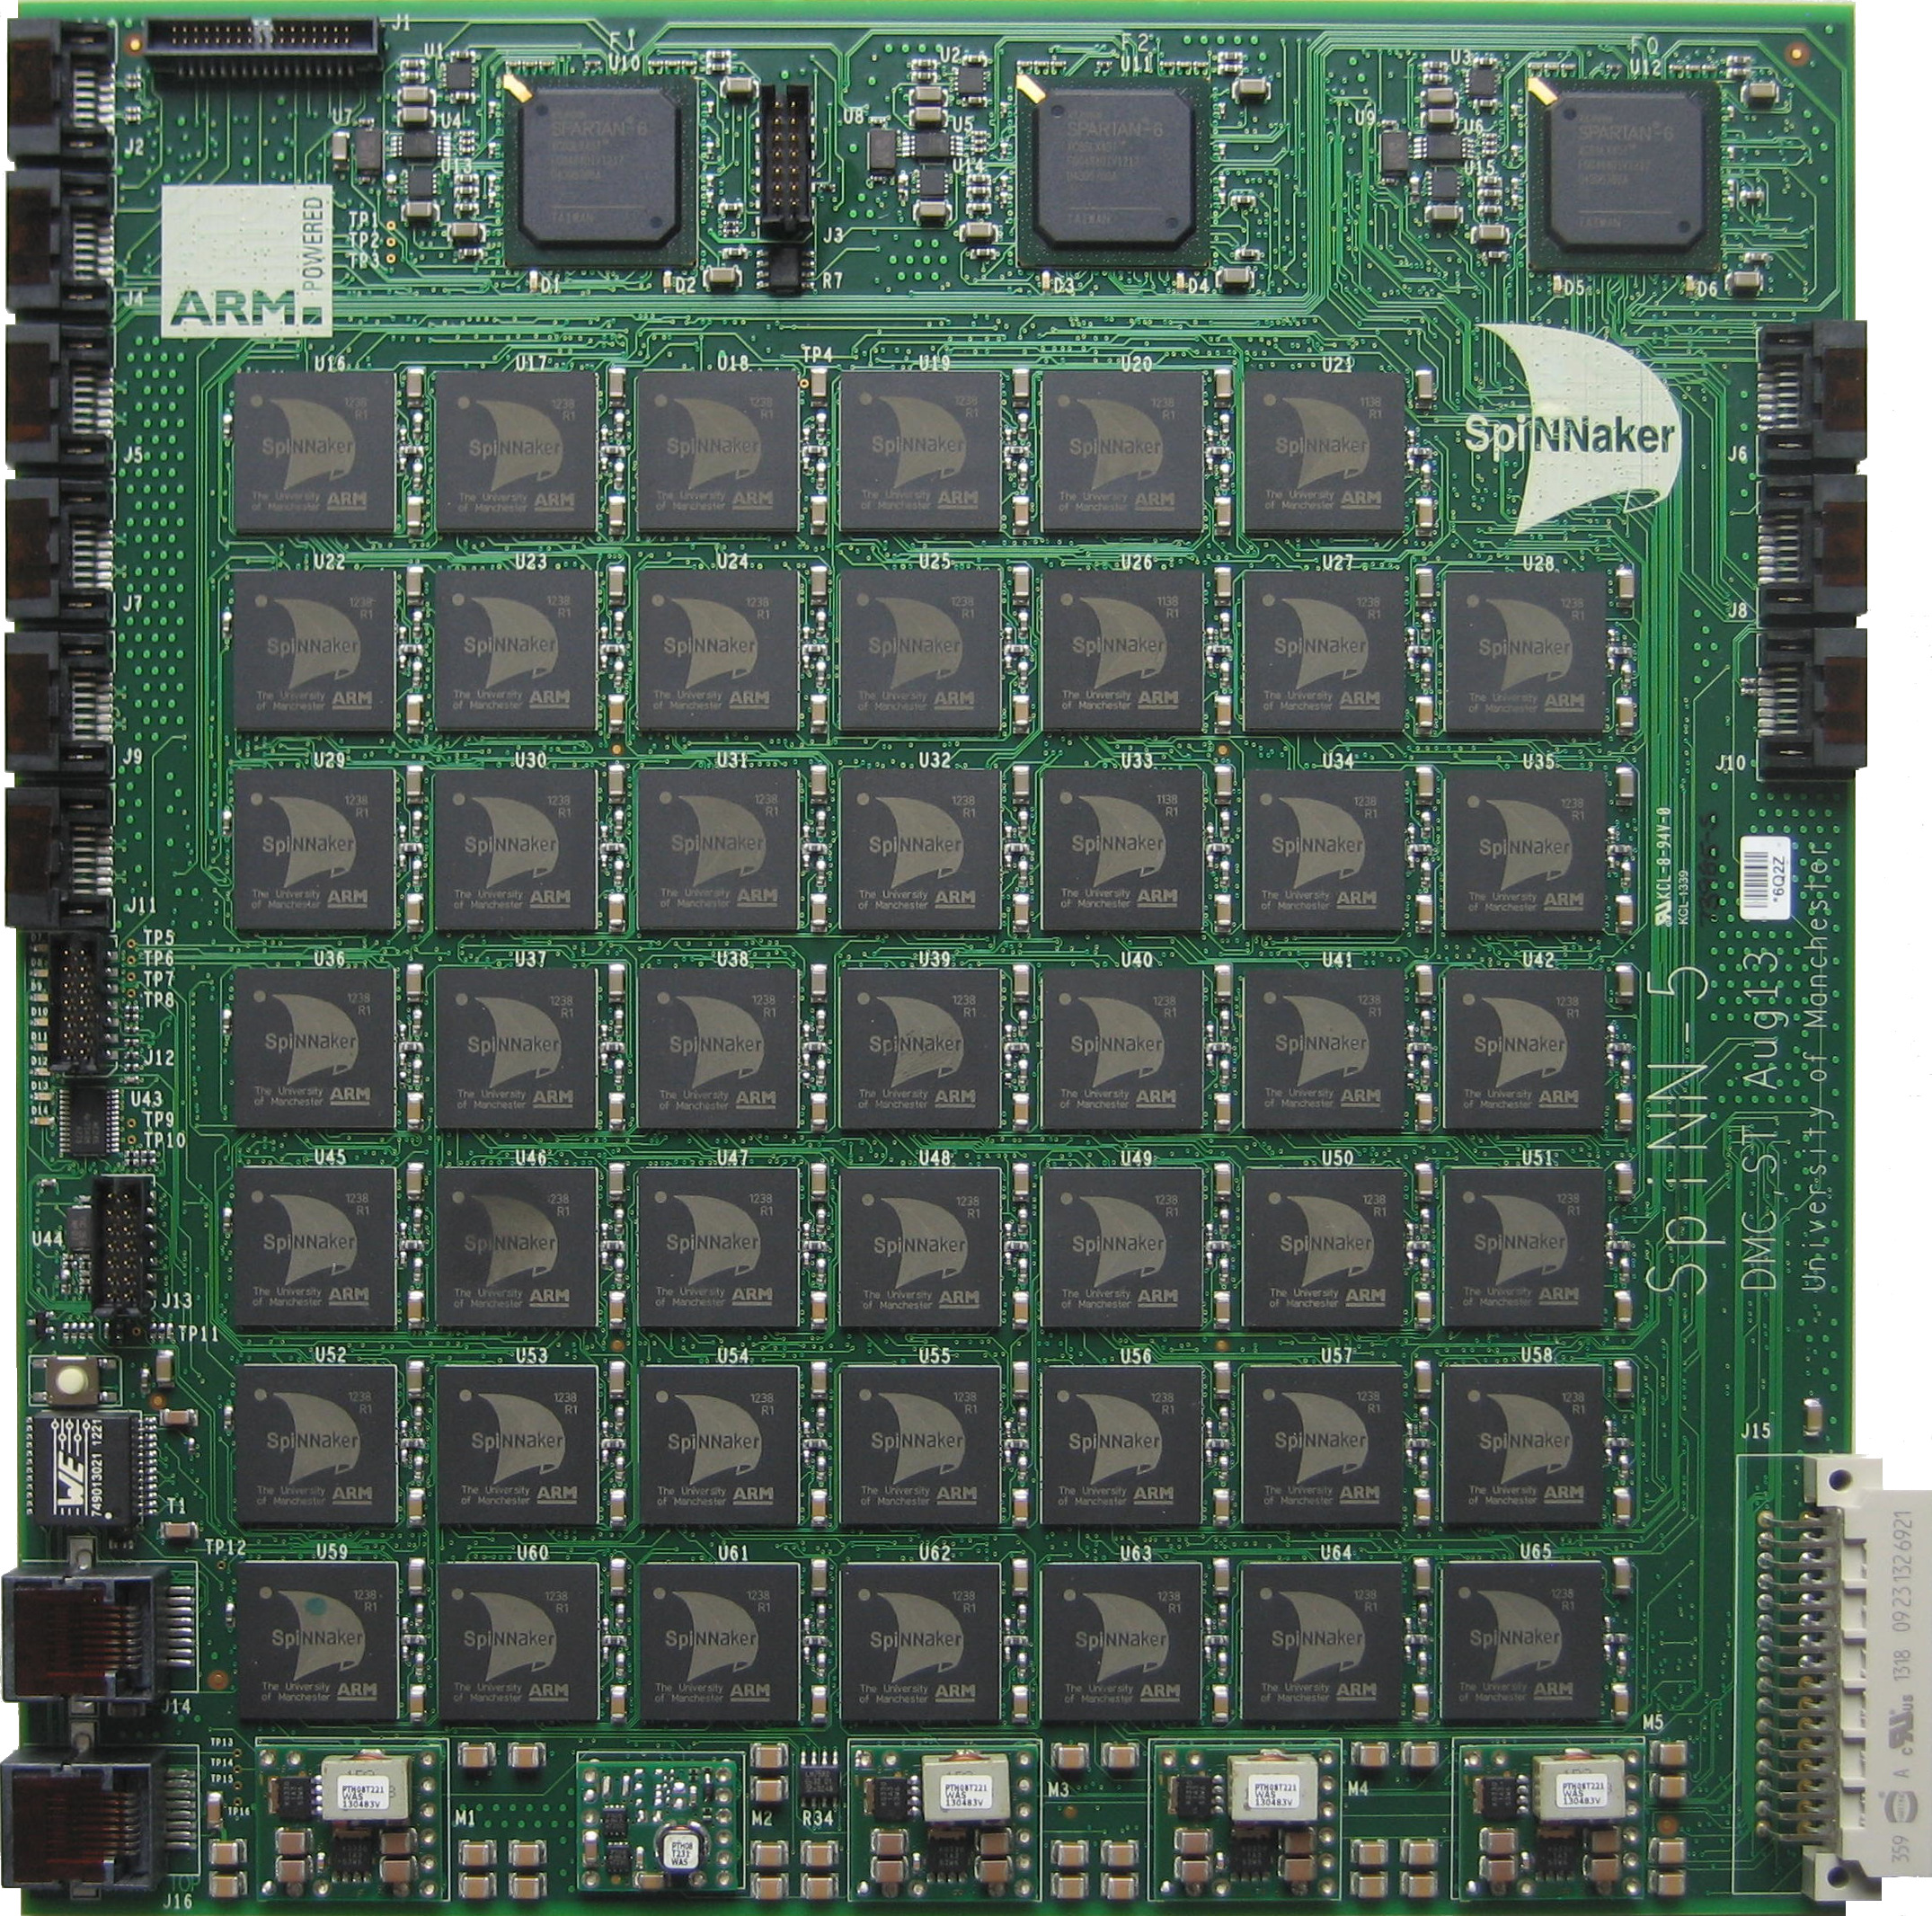
\includegraphics[width=\linewidth]{spinnakerBoard.jpg}
  \caption{A single SpiNNaker (SpiNN-5) board.
  Image reproduced with permission from Alan Stokes.}
\end{figure}

\begin{figure}[H]
  \includegraphics[width=\linewidth]
    {SpiNNaker_9cabinets.jpg}
  \caption{The SpiNNaker1M machine in Manchester.
  Image reproduced with permission from Alan Stokes.}
\end{figure}

\newpage

\section{Excerpts from the Test Suite}
\label{sec:test_suite}

\lstinputlisting[language=Python, firstline=1, lastline=68,
  caption={Excerpt from the test suite showing two models (one MLP and
    one CNN), which take up all the capacity of a SpiNN-5 board.},
  captionpos=b, numbers=left, label={lst:big_models_inference}]
  {../SpiDNN/test/test_inference.py}

\newpage

\begin{lstlisting}[language=Python, caption={Excerpt from the test
  suite showing a network similar to the MLP from
  Listing~\ref{lst:big_models_inference} being trained.
  The MLP is trained to learn XOR, so the input and output dimensions
  are different from the model shown in
  Listing~\ref{lst:big_models_inference}.
  The backward pass was implemented using shared parameters
  (see Section~\ref{subsec:problems}).}, captionpos=b, numbers=left,
  label={lst:big_mlp_training}]
import numpy as np
import tensorflow as tf

from spiDNN import Model
from spiDNN.layers import Input, Dense

from copy import deepcopy
from time import time

EPOCHS = 50
BATCH_SIZE = 4
LEARNING_RATE = 0.1

def test_mlp_backprop():
    X = np.array([[.0, .0], [.0, 1.], [1., .0], [1., 1.]])
    y = np.array([[.0, 1.], [1., .0], [1., .0], [.0, 1.]])

    kmodel = tf.keras.models.Sequential()
    kmodel.add(tf.keras.layers.Dense(
        50, activation="relu", input_shape=(2,)))
    kmodel.add(tf.keras.layers.Dense(50, activation="softmax"))
    kmodel.add(tf.keras.layers.Dense(300, activation="tanh"))
    kmodel.add(tf.keras.layers.Dense(50, activation="sigmoid"))
    kmodel.add(tf.keras.layers.Dense(25))
    kmodel.add(tf.keras.layers.Dense(2, activation="softmax"))

    kmodel.compile(
        loss="mean_squared_error",
        optimizer=tf.keras.optimizers.SGD(learning_rate=LEARNING_RATE))

    model=Model()
    model.add(Input(2))
    model.add(Dense(50, activation="relu"))
    model.add(Dense(50, activation="softmax"))
    model.add(Dense(300, activation="tanh"))
    model.add(Dense(50, activation="sigmoid"))
    model.add(Dense(25))
    model.add(Dense(2, activation="softmax"))

    model.set_weights(kmodel.get_weights())

    unfitted_weights = deepcopy(model.get_weights())

    spinn_start = time()
    model.fit(
        X, y, "mean_squared_error", epochs=EPOCHS, batch_size=BATCH_SIZE,
        learning_rate=LEARNING_RATE)
    spinn_end = time()

    keras_start = time()
    kmodel.fit(X, y, epochs=EPOCHS, batch_size=BATCH_SIZE, shuffle=False)
    keras_end = time()

    w = model.get_weights()
    w_ = kmodel.get_weights()

    error = [x - x_ for x, x_ in zip(w, w_)]
    update = [x - x_ for x, x_ in zip(w, unfitted_weights)]

    # make sure weights are updated in SDRAM before they are extracted
    for u in update:
        assert np.amax(np.absolute(u)) > 0.0

    for e in error:
        e_max = np.amax(np.absolute(e))
        print(e_max)
        assert e_max < 0.1

    print("SpiNNaker took: {} seconds".format(spinn_end - spinn_start))
    print("Keras took: {} seconds".format(keras_end - keras_start))
\end{lstlisting}

\newpage

\begin{lstlisting}[language=Python, caption={Excerpt from the test
  suite showing the training of a CNN with known weights.
  It was used for implementing backpropagation for convolutional
  layer.}, captionpos=b, numbers=left,
  label={lst:cnn_known_weights}]
import numpy as np
import tensorflow as tf

from spiDNN import Model
from spiDNN.layers import Input, Dense


def test_training_conv1d_with_known_weights():
    input_shape = (2, 1)

    X = np.array([[0., 1.]]).reshape(1,2,1)
    y = np.array([[1.]])

    weights = [
        np.array([[[.1, .4]],
                  [[.2, .5]],
                  [[.3, .6]]]), np.array([.0, .0]),
        np.array([[[ .7, 1.3],
                   [ .8, 1.4]],
                  [[ .9, 1.5],
                   [1. , 1.6]],
                  [[1.1, 1.7],
                   [1.2, 1.8]]]), np.array([.0, .0]),
        np.array([[1.9],[2.0],[2.1],[2.2]]), np.array([.0])
    ]


    c1 = tf.keras.layers.Conv1D(2, 3, padding="same", input_shape=input_shape)
    c2 = tf.keras.layers.Conv1D(2, 3, padding="same")

    kmodel = tf.keras.models.Sequential()
    kmodel.add(c1)
    kmodel.add(c2)
    kmodel.add(tf.keras.layers.Flatten())
    kmodel.add(tf.keras.layers.Dense(1))

    kmodel.compile(
        loss="mean_squared_error",
        optimizer=tf.keras.optimizers.SGD(learning_rate=1e-2))

    kmodel.set_weights(weights)

    kmodel.train_on_batch(X, y)

    model = Model()
    model.add(Input(*input_shape))
    model.add(Conv1D(2, (3,), padding="same"))
    model.add(Conv1D(2, (3,), padding="same"))
    model.add(Dense(1))

    model.set_weights(deepcopy(weights))

    model.fit(X, y, "mean_squared_error", epochs=1, batch_size=1,
              learning_rate=1e-2)

    w = model.get_weights()
    w_ = kmodel.get_weights()

    error = [x - x_ for x, x_ in zip(w, w_)]
    update = [x - x_ for x, x_ in zip(w, weights)]

    for u in update:
        assert np.amax(np.absolute(u)) > 0.0

    for e in error:
        e_max = np.amax(np.absolute(e))
        print(e_max)
        assert e_max < 0.1
\end{lstlisting}

\newpage

\begin{lstlisting}[language=Python, caption={Excerpt from the test
  suite showing the biggest CNN trained with the prototye, without
  dropped packets.}, captionpos=b, numbers=left,
  label={lst:training_cnn}]
import numpy as np
import tensorflow as tf

from spiDNN import Model
from spiDNN.layers import Input, Dense


def test_training_conv1d():
    loss = "mean_squared_error"
    kernel_size = 3
    input_shape = (10, 3)

    X = np.random.rand(4, *input_shape)
    y = np.random.rand(4, 4)

    kmodel = tf.keras.models.Sequential()
    kmodel.add(tf.keras.layers.Conv1D(
        1, 3, padding="same", input_shape=input_shape))
    kmodel.add(tf.keras.layers.Conv1D(2, kernel_size - 1, padding="same"))
    kmodel.add(tf.keras.layers.Conv1D(2, kernel_size + 2, padding="same"))
    kmodel.add(tf.keras.layers.Flatten())
    kmodel.add(tf.keras.layers.Dense(y.shape[1]))

    kmodel.compile(
        loss=loss,
        optimizer=tf.keras.optimizers.SGD(learning_rate=0.1))

    model = Model()
    model.add(Input(*input_shape))
    model.add(Conv1D(1, (3,), padding="same"))
    model.add(Conv1D(2, (kernel_size - 1,), padding="same"))
    model.add(Conv1D(2, (kernel_size + 2,), padding="same"))
    model.add(Dense(y.shape[1]))

    model.set_weights(kmodel.get_weights())

    unfitted_weights = deepcopy(model.get_weights())

    model.fit(
        X, y, loss, epochs=1, batch_size=4,
        learning_rate=0.1)

    kmodel.fit(X, y, epochs=1, batch_size=4, shuffle=False)

    w = model.get_weights()
    w_ = kmodel.get_weights()

    error = [x - x_ for x, x_ in zip(w, w_)]
    update = [x - x_ for x, x_ in zip(w, unfitted_weights)]

    for u in update:
        assert np.amax(np.absolute(u)) > 0.0

    for e in error:
        e_max = np.amax(np.absolute(e))
        print(e_max)
        assert e_max < 1.
\end{lstlisting}

\end{appendices}

\end{document}
